%作者:王美庭
%Email:wangmeiting92@gmail.com

%使用xelatex或pdflatex编译

%=============导言区===============
\documentclass[compress,10pt,dvipsnames,notheorems]{beamer} %compress表示紧缩化显示slide;beamber会自动调用xcolor宏包,dvipsnames选项表示可使用xcolor宏包对应选项的颜色名;beamer会自动加载amsthm和amsmath宏包,notheorems表示关闭beamer定义的定理类环境。
%作者:王美庭
%Email:wangmeiting92@gmail.com

%=============导言区通用设置===============

%%%=====主题设置*******
\usetheme{default} %设置整体上的主题
\usefonttheme[onlymath]{serif} %设置数学公式字体为衬线字体
%\useoutertheme{infolines}
\useinnertheme{circles}
%\usecolortheme{wolverine}
\setbeamertemplate{navigation symbols}{} %移除所有的导航栏
\setbeamertemplate{caption}[numbered] %展示图表计数器
\setbeamertemplate{footline}[text line]{\hfill\rule[-0.5em]{0pt}{1em}\insertframenumber{} / \inserttotalframenumber} %在页面右下角添加“当前帧数 / 总帧数”,\strut表示生成一个宽度为0,总高度等于行距的不可见支柱
\setbeamersize{text margin left=0.8cm, text margin right=0.8cm} %设置文字区域左右留白的宽度
\setbeamertemplate{itemize subitem}{--} %将无序列表的标志样式改为--(第二层)
%\setbeamertemplate{itemize item}[circle] %将无序列表的标志样式改为圆形(第一层)
%\setbeamertemplate{enumerate item}[circle] %将有序列表的标志样式改为圆形(第一层)
%\setbeamertemplate{section in toc}[circle] %设置section in toc为圆形包含数字


%%%=====宏包使用********
\usepackage[space=true,hyperref,UTF8]{ctex} %支持中文,加入超链接宏包,设置UTF8编码
\usepackage{graphicx} %引入图片所需宏包
\graphicspath{{figures/}} %设置图像插入路径
\usepackage{lipsum} %可输入英文假文
\usepackage{ragged2e}
\justifying\let\raggedright\justifying %设置段落对齐方式为两端对齐
\usepackage{float} %其H参数可以让浮动环境不再浮动
\usepackage{array} %提供了更多的表格列说明符,以及修正了一些表格显示上的问题
\usepackage{booktabs} %以使用学术上常见的三线表命令
\usepackage{dcolumn} %可使用小数点对齐列说明符
\usepackage{setspace}
\setstretch{1} %设置行间距的因子(默认为1)
\usepackage{calligra} %手写字体
\usepackage[T1]{fontenc} %以实现更多的字体功能,如默认字体下的斜体加粗
\usepackage{ifthen}


%设置计数器
\newcounter{mycntthm} %设置新的计数器
\newcounter{mycntexam}
\setcounter{mycntthm}{0} %设定计数器默认值
\setcounter{mycntexam}{0}


%开关设置
\newcommand{\thmseriesnamestyle}{Chinese} %Chinese表示设置定理类名称为中文,English表示设置定理类名称为英文
\newcommand{\thmseriesnumbering}{true} %true表示对定理类环境进行编号,false表示不对定理类环境进行编号

\ifthenelse{\equal{\thmseriesnamestyle}{Chinese}}{%
	\newcommand{\dfnname}{定义}
	\newcommand{\lemmaname}{引理}
	\renewcommand{\thmname}{定理}
	\newcommand{\coroname}{推论}
	\renewcommand{\proofname}{证明.}
	\newcommand{\examname}{例}
	\newcommand{\alertname}{注意}
}%
{%
	\newcommand{\dfnname}{Definition}
	\newcommand{\lemmaname}{Lemma}
	\renewcommand{\thmname}{Theorem}
	\newcommand{\coroname}{Corollary}
	\renewcommand{\proofname}{Proof.}
	\newcommand{\examname}{Example}
	\newcommand{\alertname}{Alert}
}

\ifthenelse{\equal{\thmseriesnumbering}{true}}{%
	\newcommand{\mycntthm}{\stepcounter{mycntthm}\themycntthm}
	\newcommand{\mycntexam}{\stepcounter{mycntexam}\themycntexam}
}%
{%
	\newcommand{\mycntthm}{}
	\newcommand{\mycntexam}{}
}


%自定义颜色
\colorlet{temp}{violet} %定义环境颜色
\colorlet{fgmyupdfncolor}{temp}
\colorlet{bgmyupdfncolor}{temp!20}
\colorlet{bgmylowdfncolor}{temp!10}
\setbeamercolor{myupdfncolor}{fg=fgmyupdfncolor,bg=bgmyupdfncolor}
\setbeamercolor{mylowdfncolor}{fg=black,bg=bgmylowdfncolor}

\definecolor{fgmyupthmcolor}{RGB}{51, 51, 178} %引理定理环境颜色
\definecolor{bgmyupthmcolor}{RGB}{214, 214, 239}
\definecolor{bgmylowthmcolor}{RGB}{234, 234, 247}
\setbeamercolor{myupthmcolor}{fg=fgmyupthmcolor,bg=bgmyupthmcolor}
\setbeamercolor{mylowthmcolor}{fg=black,bg=bgmylowthmcolor}

\colorlet{temp}{blue!70!orange} %推论环境颜色
\colorlet{fgmyupcorocolor}{temp}
\colorlet{bgmyupcorocolor}{temp!20}
\colorlet{bgmylowcorocolor}{temp!10}
\setbeamercolor{myupcorocolor}{fg=fgmyupcorocolor,bg=bgmyupcorocolor}
\setbeamercolor{mylowcorocolor}{fg=black,bg=bgmylowcorocolor}

\colorlet{temp}{lime!60!black} %证明环境颜色
\colorlet{fgmyupproofcolor}{temp}
\colorlet{bgmyupproofcolor}{temp!20}
\colorlet{bgmylowproofcolor}{temp!10}
\setbeamercolor{myupproofcolor}{fg=fgmyupproofcolor,bg=bgmyupproofcolor}
\setbeamercolor{mylowproofcolor}{fg=black,bg=bgmylowproofcolor}

\definecolor{fgmyupexamcolor}{RGB}{0, 127, 0} %例子环境颜色
\definecolor{bgmyupexamcolor}{RGB}{204, 229, 204}
\definecolor{bgmylowexamcolor}{RGB}{229, 242, 229}
\setbeamercolor{myupexamcolor}{fg=fgmyupexamcolor,bg=bgmyupexamcolor}
\setbeamercolor{mylowexamcolor}{fg=black,bg=bgmylowexamcolor}

\colorlet{temp}{red} %警示环境颜色
\colorlet{fgmyupalertcolor}{temp}
\colorlet{bgmyupalertcolor}{temp!20}
\colorlet{bgmylowalertcolor}{temp!10}
\setbeamercolor{myupalertcolor}{fg=fgmyupalertcolor,bg=bgmyupalertcolor}
\setbeamercolor{mylowalertcolor}{fg=black,bg=bgmylowalertcolor}


%自定义定理类环境
\newenvironment{dfn}[1][]%定义环境
{
	\begin{beamerboxesrounded}[upper=myupdfncolor,lower=mylowdfncolor,shadow]{\dfnname{} \mycntthm{} \ifthenelse{\equal{#1}{}}{}{(#1)}}\ifthenelse{\equal{\thmseriesnumbering}{true}}{\addtocounter{mycntthm}{-1}\refstepcounter{mycntthm}}{}
}%
{
	\end{beamerboxesrounded}
}

\newenvironment{lemma}[1][]%引理环境
{
	\begin{beamerboxesrounded}[upper=myupthmcolor,lower=mylowthmcolor,shadow]{\lemmaname{} \mycntthm{} \ifthenelse{\equal{#1}{}}{}{(#1)}}\ifthenelse{\equal{\thmseriesnumbering}{true}}{\addtocounter{mycntthm}{-1}\refstepcounter{mycntthm}}{}
}%
{
	\end{beamerboxesrounded}
}

\newenvironment{thm}[1][]%定理环境
{
	\begin{beamerboxesrounded}[upper=myupthmcolor,lower=mylowthmcolor,shadow]{\thmname{} \mycntthm{} \ifthenelse{\equal{#1}{}}{}{(#1)}}\ifthenelse{\equal{\thmseriesnumbering}{true}}{\addtocounter{mycntthm}{-1}\refstepcounter{mycntthm}}{}
}%
{
	\end{beamerboxesrounded}
}

\newenvironment{coro}[1][]%推论环境
{
	\begin{beamerboxesrounded}[upper=myupcorocolor,lower=mylowcorocolor,shadow]{\coroname{} \mycntthm{} \ifthenelse{\equal{#1}{}}{}{(#1)}}\ifthenelse{\equal{\thmseriesnumbering}{true}}{\addtocounter{mycntthm}{-1}\refstepcounter{mycntthm}}{}
}%
{
	\end{beamerboxesrounded}
}

\renewenvironment{proof}[1][]%证明环境
{
	\begin{beamerboxesrounded}[upper=myupproofcolor,lower=mylowproofcolor,shadow]{\proofname}
}%
{
	\hfill$\blacksquare$
	\end{beamerboxesrounded}
}

\newenvironment{exam}[1][]%例环境
{
	\begin{beamerboxesrounded}[upper=myupexamcolor,lower=mylowexamcolor,shadow]{\examname{} \mycntexam{} \ifthenelse{\equal{#1}{}}{}{(#1)}}\ifthenelse{\equal{\thmseriesnumbering}{true}}{\addtocounter{mycntexam}{-1}\refstepcounter{mycntexam}}{}
}%
{
	\end{beamerboxesrounded}
}

\newenvironment{solu}%解答环境
{
	\begin{beamercolorbox}[rounded=true,shadow=true]{mylowexamcolor}
}%
{
	\end{beamercolorbox}
}

\renewenvironment{alert}[1][]%警示环境
{
	\begin{beamerboxesrounded}[upper=myupalertcolor,lower=mylowalertcolor,shadow]{\alertname}
}%
{
	\end{beamerboxesrounded}
}
 %插入导言区设置
\usepackage{tikz}
\usetikzlibrary{shapes,arrows}
\usepackage{caption}

%标题页设置
\title{完备统计学习理论}
\subtitle{——统计学批判和统计学习理论的阐述}
\author{席泽璞}

%\date[\today]{\small \today}

%%有多位作者时:
%\author[张三,李四]{张三\inst{1} \and 李四\inst{2}}
%\institute[IESR-JNU, SOE-HUST]
%{
%	\inst{1}\textcolor[rgb]{0.0,0.0,0.1}{\small\ttfamily 经济与社会研究院,暨南大学}
%	\and
%	\inst{2}\textcolor[rgb]{0.0,0.0,0.1}{\small\ttfamily 经济学院,华中科技大学}
%}





%=================正文区=================
\begin{document}
	
\begin{frame}[plain,noframenumbering] %标题页帧
	\titlepage
\end{frame}

{
\setbeamertemplate{footline}{} %临时置空footline
\begin{frame}[noframenumbering]{目录} %大纲,[pausesections]表示动态一步一步显示,[hideallsubsections]表示隐藏所有的subsection,[hideothersubsections]表示隐藏非当前节下的subsection,[currentsection]表示只正常显示current section,而虚化其他的section
	\tableofcontents[hideallsubsections]
\end{frame}
}

% 在每一section的开头插入以下内容
\AtBeginSection[]{ % 不对section*起作用
	{\setbeamertemplate{footline}{} %临时置空footline
	\begin{frame}[noframenumbering]{}
		\tableofcontents[currentsection,hideothersubsections]
	\end{frame}}
}


\section{第一章 研究对象和地位}
\begin{frame}{第一章 研究对象和地位}
\begin{figure}
\centering
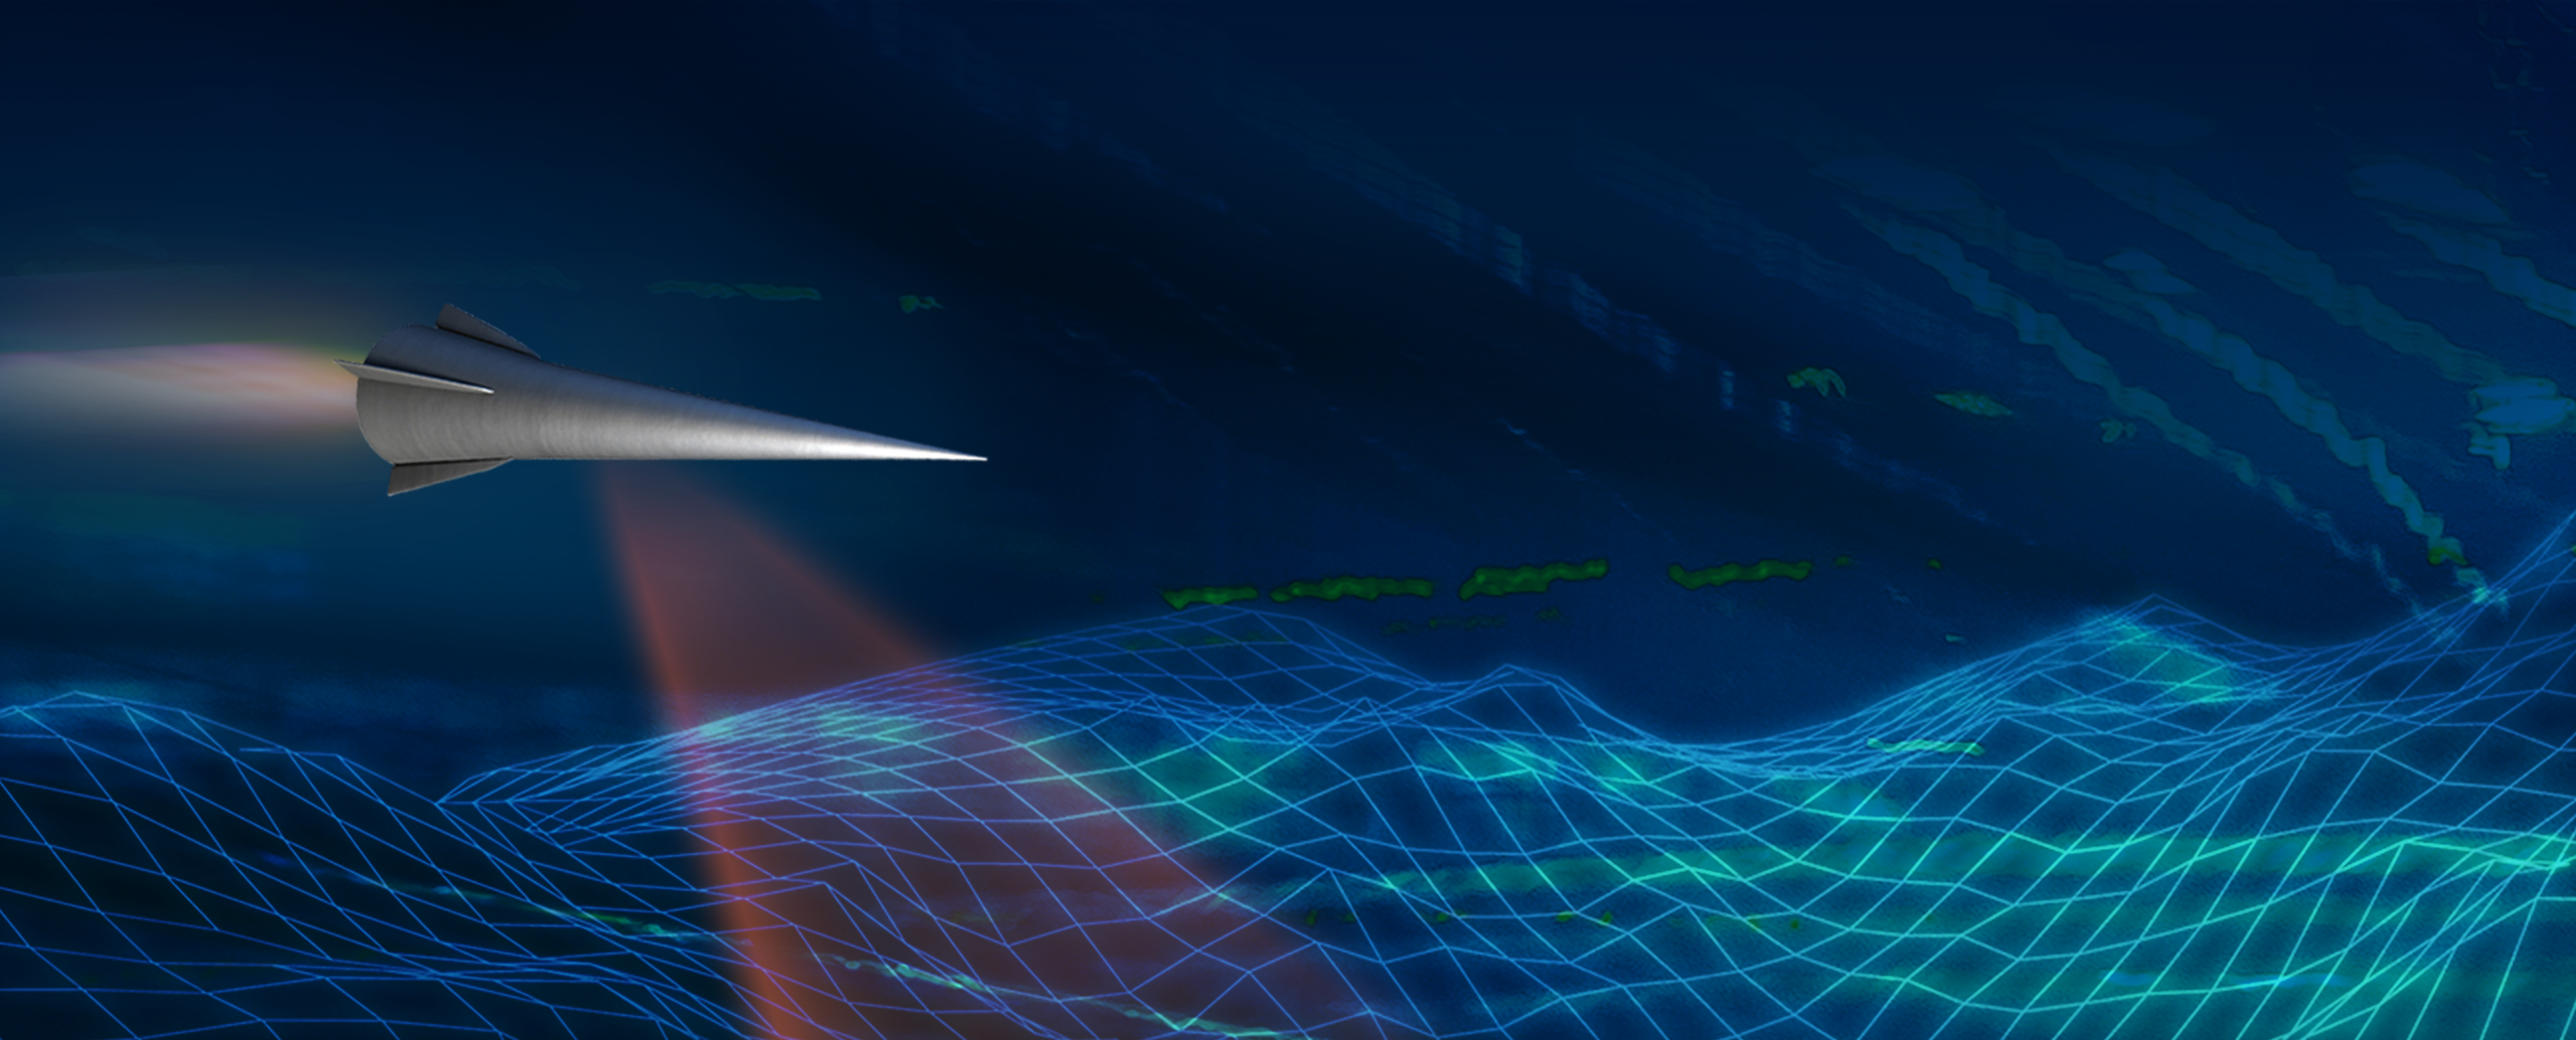
\includegraphics[width=.5\linewidth]{Imgs/mission-campaign.png}
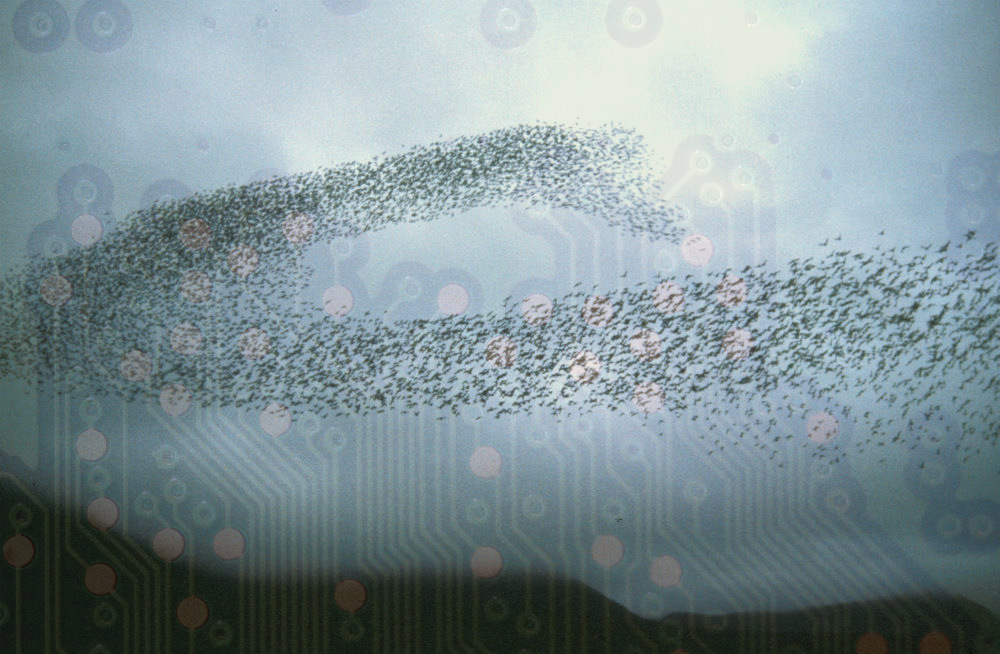
\includegraphics[width=.5\linewidth]{Imgs/Swarm-2.jpg}
\end{figure}
\begin{solu}
\begin{enumerate}
\item 这类问题都是模式识别问题.
\item 如何在哲学上把握学习理论的优越性.
\item 如何在存在论(ontology)上把握学习理论对当前一般知识样式的革命.
\end{enumerate}
\end{solu}
\end{frame}

\begin{frame}
\begin{figure}
\centering
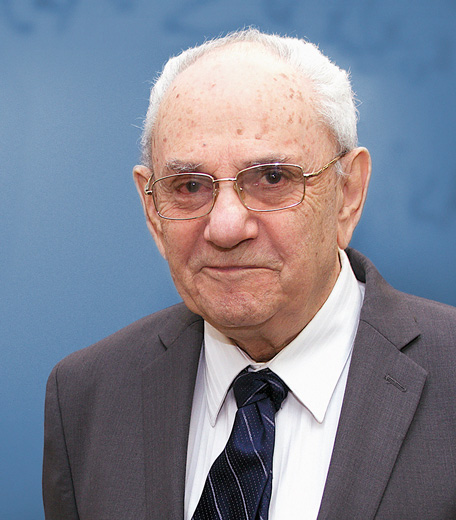
\includegraphics[width=.5\linewidth]{Imgs/vladimir-vapnik-456x520-1.jpg}
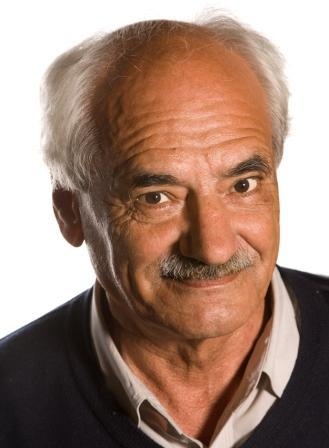
\includegraphics[width=.45\linewidth]{Imgs/chervonenkis_from_wiki.jpg}
\captionsetup{labelformat=empty}
\caption{Vladimir N. Vapnik(1936年12月6日-) Alexey Ya. Chervonenkis(1938年9月7日-2014年9月22日)}
\end{figure}
\end{frame}

\begin{frame}
\begin{figure}

\includegraphics[width=.3\linewidth]{Imgs/TheoriederZeichenerkennung.jpg}
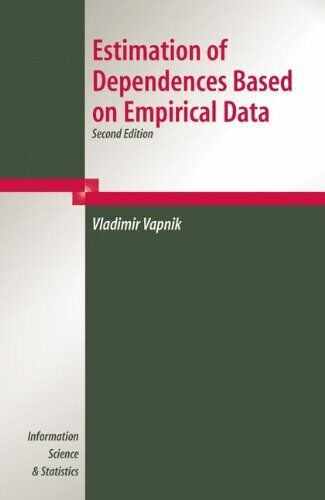
\includegraphics[width=.27\linewidth]{Imgs/EDBED1982.jpg}

\includegraphics[width=.27\linewidth]{Imgs/vapnik1984.jpg}
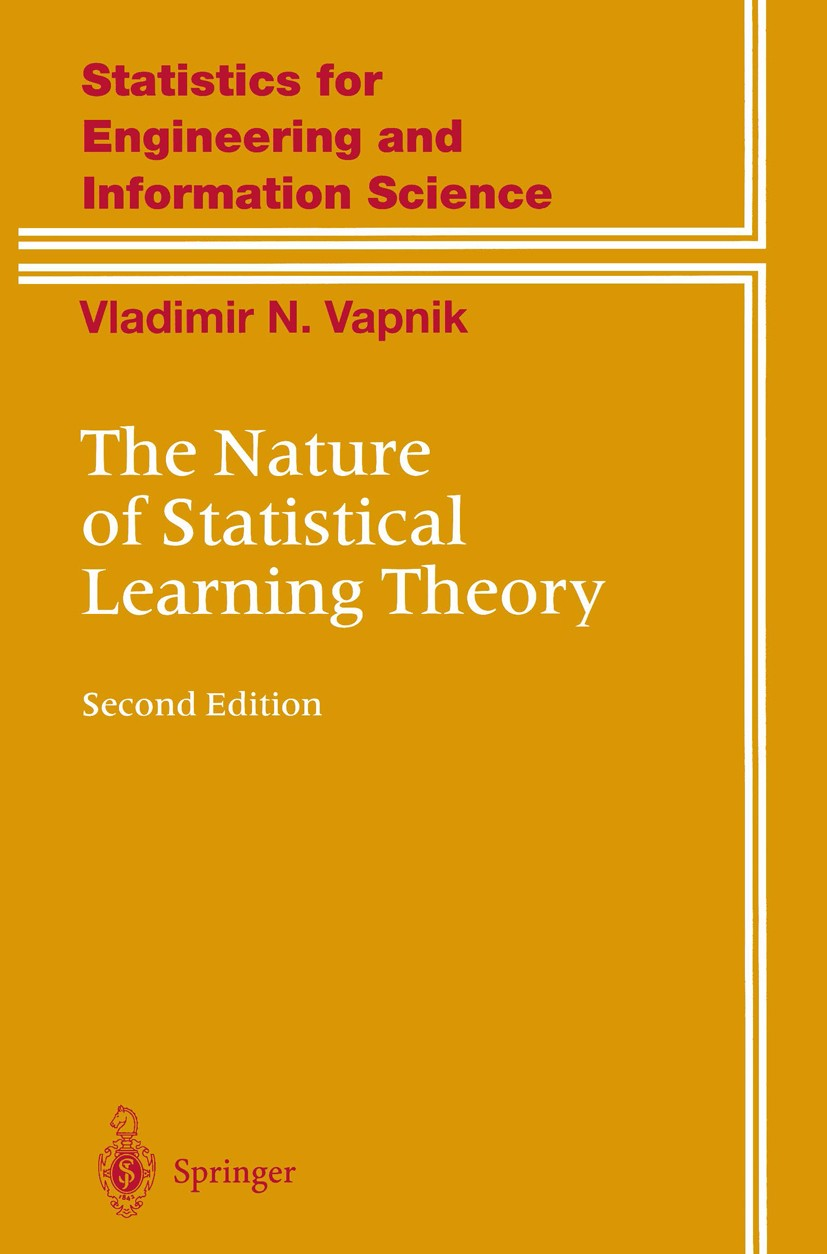
\includegraphics[width=.28\linewidth]{Imgs/nature.jpg}
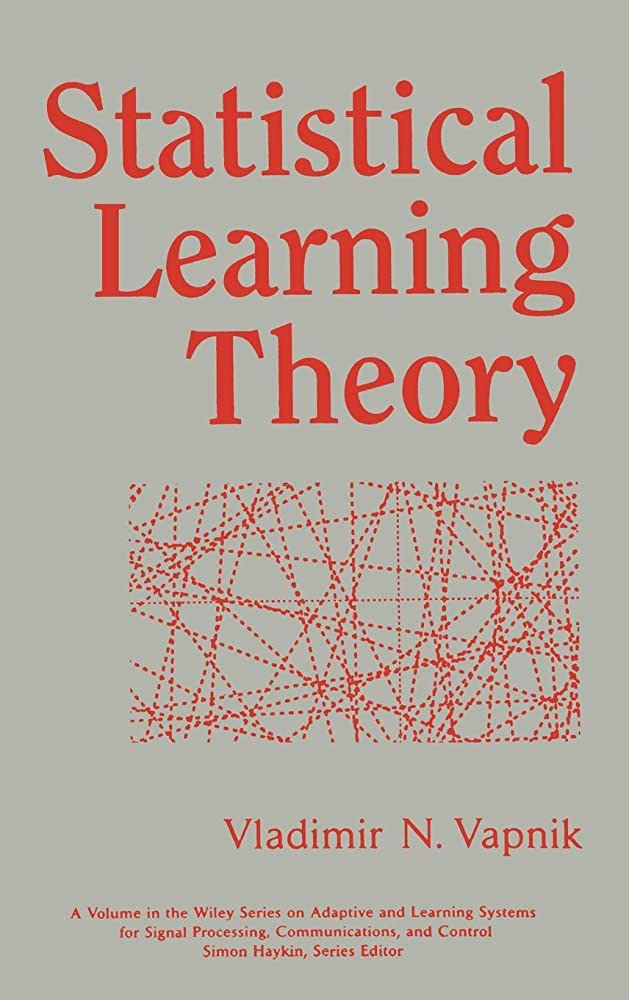
\includegraphics[width=.27\linewidth]{Imgs/STL.jpg}
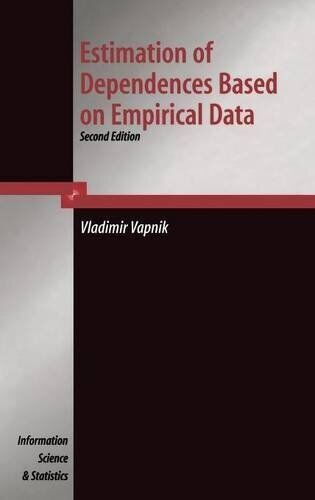
\includegraphics[width=.27\linewidth]{Imgs/EDBED.jpg}

\end{figure}
\end{frame}

\begin{frame}
\begin{figure}
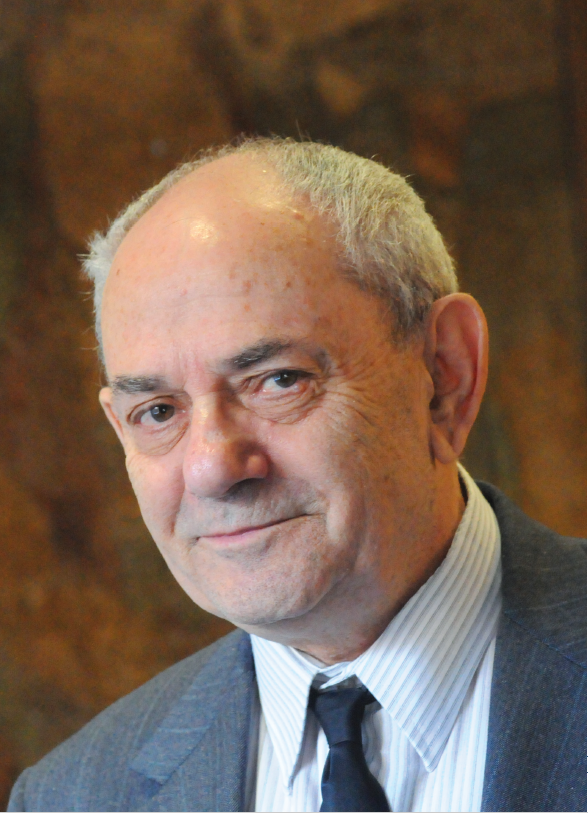
\includegraphics[width=.5\linewidth]{Imgs/vapnik.png}
\captionsetup{labelformat=empty}
\caption{Vladimir N. Vapnik}
\end{figure}
\end{frame}

\begin{frame}{第一章 研究对象和地位}
\begin{solu}
\begin{enumerate}
\item Vapnik and Chervonenkis (1974): 《Theory of Pattern Recognition》的副标题不能忘记: “Statistical Problems of Learning”. 1979年德文版问世, 至今无英译本.
\item Vapnik (1979) 《Estimation of Dependences Based on Empirical Data》, 1982年英译本问世.
\item Vapnik (1995) 《The Nature of Statistical Learning Theory》, 1998年中译本 《统计学习理论的本质》 张学工译
\item Vapnik (1998) 《Statistical Learning Theory》, 2000年中译本《统计学习理论》 许建华、张学工译
\item Vapnik (2006)  《Estimation of Dependences Based on Empirical Data》, 2006年为1982版写了《Empirical Inference Science》后记.
\item Vapnik和Chervonenkis是关于学习理论的真正奠基者, 没有之一. 对这两位大思想家关于学习问题的哲学阐述, 到现在为止仍然是空白.
\item 对这两位大思想家哲学的阐述, 根本不局限在我个人的兴趣所至, 而是我们这个时代的必然要求. 不懂VC Theory的核心, 就不可能在根基上, 在存在论的基础上, 真正理解并且把握何谓学习问题.
\end{enumerate}
\end{solu}
\end{frame}

\begin{frame}{第一章 研究对象和地位}
请回答下列几个问题:

\begin{solu}
\begin{enumerate}
\item 诚恳说来, 似乎大多数研究者都觉得“把网络搞得深深的、把层数搞得多多的”这点似乎确实不是那么的简洁、不是那么地像科学.
\item 为什么SVMs 的原文标题是“Support Vector Networks” 但Vapnik 一直使用“Support Vector Machines”, 并且在严肃阐述问题时Vapnik 一直用“SVMs”而不是“SVM”? 难道使用“SVMs”这样的复数形式仅仅是语法学层面的要求吗?
\item Vapnik 本人怎么批判地看待“网络”和“机器”的区别和联系呢?
\item 为什么在2014 年Vapnik 竟然给出“学习才刚刚开始”这样的陈述?
\item 2015 年的时候(那时候可是几乎人人都像现在一样口口声声言说“人工智能”的时候)Vapnik 竟然给出“支持向量机是暴力算法”这样的陈述?
\item 如果我们细心阅读就会发现Vapnik 直到2015年以后才明确给出“智能学习”(更准确说来应该是“智慧学习”) 的陈述. 难道我们以前的工作在Vapnik 看来都不算“智能学习”理论吗?
\item 怎么理解Vapnik 所言的“暴力”呢? Vapnik 所言的“智慧”又所指何物
呢?
\end{enumerate}
\end{solu}
\end{frame}


\begin{frame}{第一章 研究对象和地位}
\begin{solu}
\begin{enumerate}
\item 如果我们能够这样追问问题, 那么我们其实就进入“哲学的思”.
\item 在哲学家看来, 有两种思维方式: 一种是“{\color{red}{自然的思}}”, 就是不去追问这个事情的前提条件, 我们仅仅在此前提下从事知识的获取; 另一种是“{\color{red}{哲学的思}}”, 即批判. 批判的思总是需要追问让事物如此这般的前提是什么.
\item {\color{red}{本论文讨论的是“哲学的思”.}} 我们不会在统计学的框架内进行技术的探究, 我们要追问让统计学成为可能的前提条件是什么; 统计学的前提条件和学习理论——例如神经网络——有没有区别.
\pause
\item {\color{red}{本论文的目的是揭示统计学思想上的天真和无头脑.}}
\pause
\item {\color{red}{本论文的不是通过我自己的话来解释统计学的无头脑, 而只不过是翻译了一下统计学家自己的语言而已, 但是为何国内的所谓那些著名统计学家们要沉默呢?}}
\pause
\item {\color{red}{本论文并不想叫醒那些沉睡的统计学家, 而是为我们自己搞清楚问题, 以便使得我们自己不要再错下去}}.
\item {\color{red}{要做到这一点极其艰难, 不仅仅是因为我先前所受的教育正就是统计学, 更大的原因是此论文标示着一种和当下主流知识类型的决断.}}
\item {\color{red}{实现的这一目的的方法是对比统计学与统计学习理论.}}
\end{enumerate}
\end{solu}
\end{frame}

\begin{frame}{第一章 研究对象和地位}
\begin{solu}
\begin{enumerate}
\item 当然我们也必须估计到, 以上的这段陈述肯定会引起反对的意见和可预见的反感.
\item 完全可以想象对于统计学习理论的哲学层面上的阐述, 似乎就必定是一种徒劳.
\pause
\item Vapnik 本人对类似这样的徒劳都是知晓的. Vapnik 本人不止一次的惊讶地表达过, 有时候也离奇地反问过人们到底有没有真切地去了解过统计学习理论.
\item 人们仅仅是草草地用一下在统计学习理论指导下开发的SVMs 算法就了事了,然后就把这个工具轻松地扔掉了, 并且很大程度上扔在统计学那边去了.
\pause
\item 我们以上的陈述不可能发生在统计学的博士论文中, 但是对于计算机专业的博士生, 似乎是有希望的.
\item 就像Vapnik 本人所言“统计学习理论在统计学那里没有找到自己的家, 统计学习理论是在计算机科学领域找到了自己的家.”
\pause
\item 因为“博士研究生”的全称——“哲学博士研究生”——还没有抛弃“哲学”二字, 所以我想{\color{red}{冒险一试}}, 这一冒险试图将Vapnik 本人“含蓄地”表达过了的思想内容做出一些陈述. 这些内容按照Vapnik本人的话{\color{red}{“是比技术更加重要的”}}.
\end{enumerate}
\end{solu}
\end{frame}


%\begin{frame}
%\begin{solu}
%\begin{enumerate}
%\item 
%\end{enumerate}
%\end{solu}
%\end{frame}

\begin{frame}{第一章 研究对象和地位}
\begin{solu}
\begin{enumerate}
\item 自1930s至今, 主流的知识类型都是由R.A. Fisher的统计学所规定的, 这种思想是人们处理数据的基本方法.
\item 统计学处理数据的流程是:
模型 - 数据 - 模型
\item 统计学的模型{\color{red}{由观测变量直接组成, 只是组合系数未知}}. 一切都围绕最小二乘的思想展开
\begin{align*}
Y = X\beta + \epsilon
\end{align*}
\end{enumerate}
\end{solu}
\begin{figure}
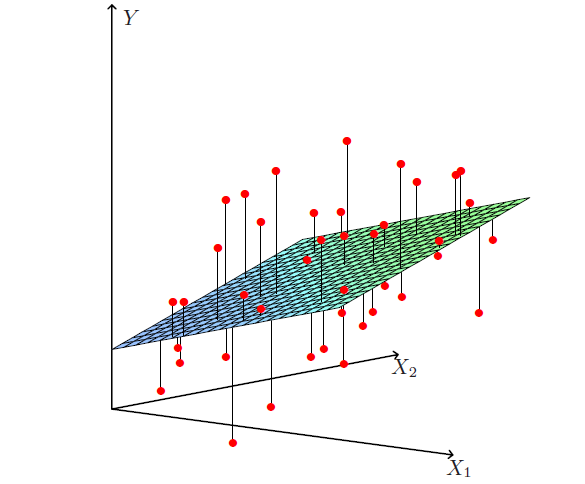
\includegraphics[width=.4\linewidth]{Imgs/least-square.png}
\captionsetup{labelformat=empty}
\caption{统计学认为数据的规律: 最小二乘}
\end{figure}
\end{frame}


\begin{frame}{第一章 研究对象和地位}
\begin{solu}
\begin{enumerate}
\item 神经网络: 颠覆性技术出现在1958年由Frank Rosenblatt制造出的感知机(Perceptron). 由于物理连接, Rosenblatt仅能手动控制最后一层.
\end{enumerate}
\end{solu}
\begin{figure}
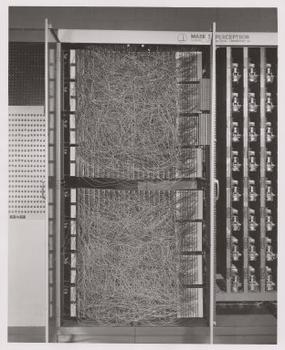
\includegraphics[width=.3\linewidth]{Imgs/Mark_I_perceptron.jpeg}
\captionsetup{labelformat=empty}
\caption{第一台感知机: {\color{red}{神经网络是科学、并且是颠覆性科学}}}
\end{figure}
\begin{solu}
\begin{enumerate}
\item 感知机的数学原理: Novikoff 1962年证明这台{\color{red}{完全受神经学研究启发下制造出来的}}感知机, 本质上是将经验数据投射到某个{\color{red}{抽象数学空间}}, 在数学空间中构建了超平面实现模式识别的.
\end{enumerate}
\end{solu}
\end{frame}

\begin{frame}{第一章 研究对象和地位}
\begin{solu}
\begin{enumerate}
\item 什么叫“数学空间”.
\begin{enumerate}
\item 柏拉图主义: 真理在理念世界、事物(Things)是对理念世界不完善的模仿
\item 笛卡尔: “我思故我在”. 建立正交坐标系. -> 牛顿: 观测量作为正交坐标
\item 康德: 纯粹理性. Hilbet: 纯粹理性下正交函数建坐标.
\item 傅里叶: 坐标使用纯粹理性的正交三角函数
\item Kolmogorov(苏联): \textbf{独立随机变量}和\textbf{正交函数}性质一样 -> 概率论.
\end{enumerate}
\item 自从Hilbert之后, 原则上只要谈及“数学空间”肯定唯一指的就是“纯粹理性抽象数学空间”, 而不是由经验观测变量组成的.
\item Kolmogorov概率论打开了历史唯物主义与唯心主义对立的开端.
\item Novikoff (1962) 证明之后事情是清楚了的: 神经网络之所以能具有学习能力, 并不是什么模拟人脑, 并不是什么突触、神经元这样的模棱两可的词汇, 它就只不过是用机器实现了某个数学空间.
\item Rosenblatt把最后一层旋转了一下(当时的硬件条件限制, 那时候是模拟计算机, 不是数字计算机), 只不过相当于变换了一下数学空间.
\end{enumerate}
\end{solu}
\end{frame}

\begin{frame}{第一章 研究对象和地位}
\begin{solu}
\begin{enumerate}
\pause
\item 我们不可否认, 人类关于飞行的研究的确受到过鸟类飞行的启发; 但是对于飞行真正的研究,那是{\color{red}{空气动力学的事业}}.
\pause
\item 我们不可否认, 人类关于学习的研究的确受到过神经学研究的启发; 但是对于学习真正的研究, 那是{\color{red}{统计学习理论的事业}}.
\item 我们不可否认, 人类关于集群行为的研究的确受到过自然界群体动物的启发; 但是对于集群行为真正的研究, 那是{\color{red}{统计学习理论的事业}}.
\pause
\item 并不是{\color{red}{统计学习理论}}规定了学习事业, 而是说{\color{red}{统计学习理论}}只不过是人类在学习历史上人民生活的一次完整理论表达.
\item 而对学习理论的研究必须破除统计学思维范式. 因此, 本文的第一部分在内容上是批判的, 在阐说的目的上是为了让我们摆脱统计学思想的干扰. 这里的提示不是个人的兴趣, 而是我们自己终于发现我们错了之后, 诚实的研究所得的结论.
\pause
\item 本文的第二部分是在第一部分阐述基础上展开的应用研究. 一旦思想的事业得以阐述清楚, 应用的工作就非常简单. 
%\item “理论一经群众掌握就会变成强大的物质力量.” —— 马克思
\end{enumerate}
\end{solu}
\end{frame}




%\begin{frame}{统计学处理问题的思想}
%\begin{figure}
%\centering
%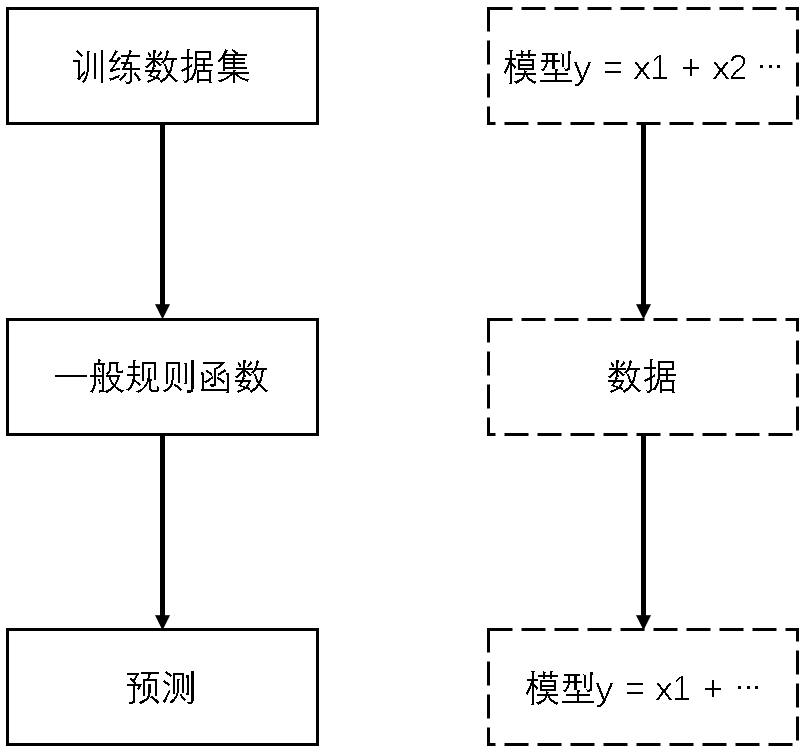
\includegraphics[width=.5\linewidth]{Imgs/statistics.png}
%\end{figure}
%\begin{solu}
%针对“基于经验数据的相依关系估计问题”我们目前接受的所有教育都是基于1930s由R.A Fisher给出的\textbf{统计学}研究思想: 即我们如何从零散的数据中提出类似规律的问题.
%\end{solu}
%\begin{solu}
%\begin{enumerate}
%\item 在统计学思想下, 我们首先假设数据中存在某种规律(某客体函数), 这种规律由直接观测变量线性组合而成, 只是组合系数未知;
%\item 统计学家利用各种统计学方法计算组合系数;
%\item 利用计算得到的组合系数, 就得到一个一般的规则函数;
%\item 利用得到的一般函数再去预测.
%\end{enumerate}
%\end{solu}
%\end{frame}
%
%\begin{frame}{计算机出现后真实的数据处理流程}
%\begin{figure}
%\centering
%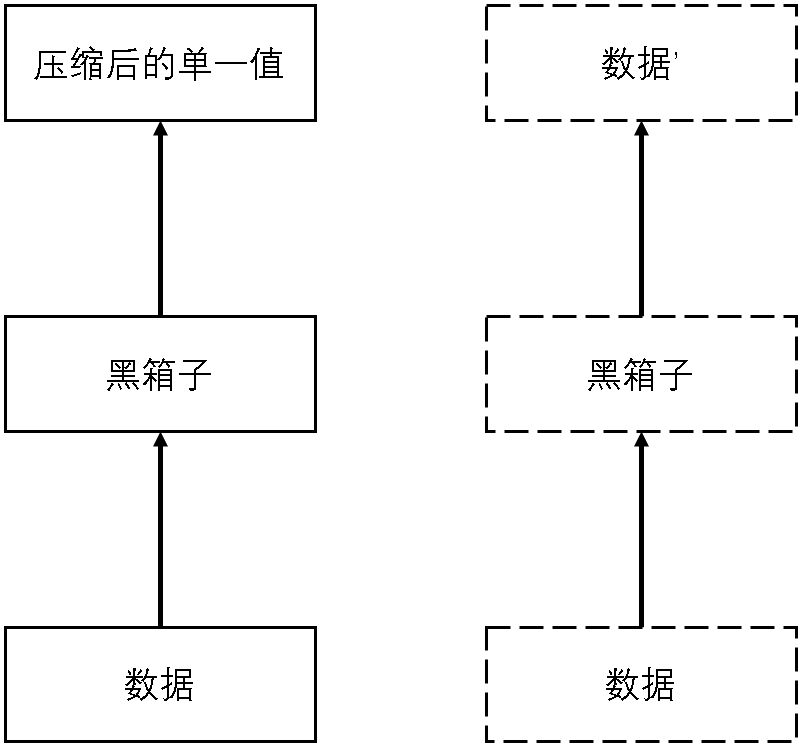
\includegraphics[width=.5\linewidth]{Imgs/ML.png}
%\end{figure}
%\begin{solu}
%\begin{enumerate}
%\item 计算机出现后(神经网络), 我们不需要假设数据中存在某种规律;
%\item 计算机工程师构建复杂的黑箱子(神经网络、深度学习);
%\item 利用机器输出的压缩后的单一值做决策;
%\end{enumerate}
%\end{solu}
%\end{frame}
%
%\begin{frame}{如何理解两个流程的本质区别}
%\begin{figure}
%\centering
%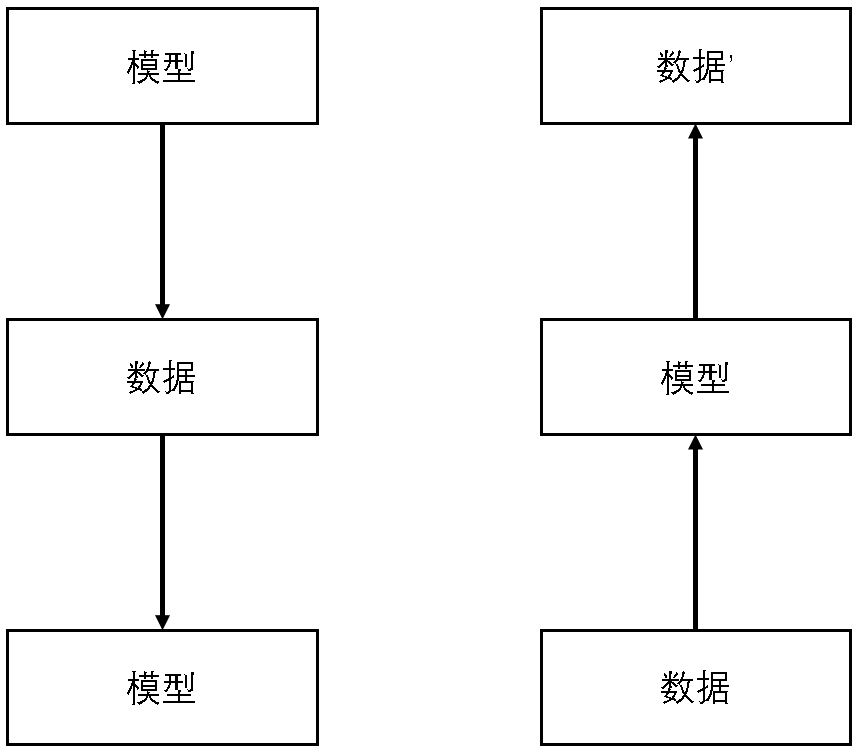
\includegraphics[width=.5\linewidth]{Imgs/statisticsVSmachinelearning.png}
%\end{figure}
%\begin{solu}
%\begin{enumerate}
%\item 如何理解这两种不同数据处理流程的本质区别;
%\item 这里所言的“本质区别”是在哲学根基上的不同;
%\item 在第二种处理流程中统计学习理论到底给我们传递了什么.
%\end{enumerate}
%\end{solu}
%\end{frame}
%
%\begin{frame}
%\begin{solu}
%\begin{enumerate}
%\item 我们在本论文中展开的是\textbf{统计学批判}和\textsf{统计学习理论}(Statistical Learning Theory, 也称作Vapnik-Chervonenkis理论)阐述的研究.
%\item “批判”不是全盘否定, 而是“阐明前提, 划定界限”.
%\item 统计学批判研究\textbf{不是}个人兴趣所至, 而是在面对机器学习已然在各个领域推进后, 对这种新知识类型的哲学认识是必然的要求, 我们必须破除以往以统计学为标本的知性科学思想, 方才能理解学习问题本身.
%\item 对统计学批判并\textbf{不是}我本人的首创, Vapnik在自己的著作中已经含蓄地明确表达过并且一直在表达这件事. 但是人们都哲学层面和思想层面不会有任何一丝的进展.
%\item 统计学批判无论是技术上(主要与p-值有关、与科学可重复性有关)还是美国统计学会和能思的统计学家们, 都对统计学展开着怀疑. 但是他们从来没有在哲学上、在根基上、在统计学成为可能的那个前提层面给出本文的阐述.
%\item 本文的阐说不仅仅是言说, 更加重要的是这样的阐说是直接服务于技术开发的. 通过对统计学批判的阐说, 我们就能够更深层次理解Vapnik, 也能更深层次理解何谓机器学习, 也就能理解为什么我们在博士期间要做机器学习的不确定量化.
%\end{enumerate}
%\end{solu}
%\end{frame}

\section{第二章 统计学的贫困}
\begin{frame}{第二章 统计学的贫困}
\begin{solu}
\begin{enumerate}
\item 我是在颇为不安地反思如何真切地辨明统计学与机器学习——最初是基于神经网络相关的机器学习——这两种知识类型的本质区别而展开研究的. 

\item 我一直是在统计学的框架下展开可信学习问题(这与硕士研究的经历密不可分), 在这个框架下我研究的内容最后归结于如何获得有效的p-值. 直到2020年10月开始关注Conformal Prediction方法, 因为这个方法能够自动保证p-值有效. 

\item 可以想见, 在先前那两三年的疑虑和困惑的停留中, Conformal Prediction方法为我开启了一种格外明朗的光照, 此光照起初在技术上的炫目让我深为服膺. 也正是在深入到Conformal Prediction方法细节研究的时候——即如何理解非一致性得分函数——我真正开始阅读Vladimir Vapnik的著作.
\end{enumerate}
\end{solu}
\end{frame}

\begin{frame}{第二章 统计学的贫困}
\begin{solu}
\begin{enumerate}
\item 我视图从理论上深入地理解Vapnik统计学习理论哲学. 

\item 在我看来, Vapnik统计学习理论哲学唯有通过阅读Vapnik原著才能得以可能, 但是真正读懂Vapnik原著又需要读者自己发动革命. 这就给我们一个很有意思的循环: 要读懂Vapnik统计学习理论就需要Vapnik统计学革命思想, 而Vapnik统计学革命思想又在Vapnik统计学习理论中. 

\item 正就是在这样一种理解下我开始阅读Vapnik的原著, 通过阅读原著我的思想发生了彻底的转变. Vapnik发动的统计学革命虽然在计算机领域的前沿研究中都得到了技术上的认可——这种认可更多由计算机领域的专家们以含蓄的技术阐述言说——但是在哲学的基础方面却并没有得到澄清, 甚至并未被真正研究过. 
\end{enumerate}
\end{solu}

%\begin{alert}
%为什么要用“贫困的统计学”和“统计学的贫困”?
%\begin{enumerate}
%\item 蒲鲁东: 《贫困的哲学》
%\item 马克思: 《哲学的贫困》
%\end{enumerate}
%\end{alert}
\end{frame}

\begin{frame}{2.1 贫困的统计学}
\begin{solu}
\begin{enumerate}
\item 我们就完全可以估计到, 在统计学盛行的当下, “贫困的统计学”这个题目一定会引起反对意见. 
\item 统计学的杰出代表, 斯坦福大学统计系终身教授 Bradley Efron 就一定会反对我的看法. 他在2001年对对 Breiman(2001)极为不屑的的评论和他本人Efron(2020)的阐述就能看到这样的反对意见.
\item 他说:“我第一次瞥了一眼Leo Breiman 这么刺激的文章后发现他似乎是反对精简吝啬法则和科学本身
的洞察力的, 而是支持那伴随着密密麻麻的旋转按钮的黑盒子模型. 而当我再一次瞥了那文章之后发现仍然
是这个路数, 但这文章本身确实是刺激得很, 我们必须要把Leo 本人的那些重要的观点给敲打敲打并且给一
一讲清楚.”(原文: “... and Leo has some important points to hammer home.”)
\item 贫困 = {\color{red}{统计学真正的科学性}}——即它为自己提出科学任务以及实现这些科学任务而制定的方法论、开发的工具——{\color{red}{已经成为不可能了.}}
\end{enumerate}
\pause
\begin{enumerate}
\item 统计学是知性科学
\item 统计学错把坐标当维数
\item 统计学理解的概率不是概率
\item 统计学给出的结果都是应诺
\end{enumerate}
\end{solu}
\end{frame}

\begin{frame}{2.1.1 统计学是知性科学}
\begin{solu}
\begin{quotation}
(Moore et al., 2000):
“至少在统计学家们看来, 统计学是一门数学科学, 但它不是数学的一个子领域. 我们统计学家们甚至用格言律令就表明我们的科学和数学是有区别的: George Box就说:‘所有的模型都是错的, 但是有一些模型是有用的’. George Cobb 就说:‘在数学领域, 内容是遮掩着结构的. 而在数据分析领域, 内容则提供意义.’David Moore 就说: ‘数学的那些定理都是为真的; 而统计的那些方法当使用某些技巧的时候都是高效率的.’”
\end{quotation}
\end{solu}
(Moore et al., 2000)的两个标题:

\begin{solu}
\begin{enumerate}
\item “统计学是与众不同的”(Moore et al., 2000, p. 2)
\item “统计学, 唉, 你确实是与众不同的啊”(Moore et al., 2000, p. 6).
\end{enumerate}
\end{solu}
这是美国统计学家(并且是著名统计学家)自己反思自己所说的话.
\end{frame}

\begin{frame}{2.1.1 统计学是知性科学}
\begin{solu}
\begin{quotation}
恩格斯在《资本论》第二卷·序言写到:

“大家知道, 直到前一世纪末, 燃素说还处于支配的地位. 根据这种理论, 一切燃烧的本质都在于从燃烧物体中分离出一种另外的、假想的物体, 即称为燃素的绝对燃烧质. 这种理论曾足以说明当时所知道的大多数化学现象, 虽然在某些场合不免有些牵强附会. ...”

“但到1774年, 普利斯特列析出了一种气体, ... 他称这种气体为无燃素气体. ... 过了不久, 瑞典的舍勒也析出了这种气体, ... 他称这种气体为火气. ...  ”

“普利斯特列和舍勒析出了氧气, 但不知道他们所析出的是什么.他们为“既有的”燃素说“范畴所束缚”

“当时在巴黎的普利斯特列立刻把他的发现告诉了拉瓦锡, 拉瓦锡就根据这个新事实研究了整个燃素说化学, 方才发现:这种新气体是一种新的化学元素; 在燃烧的时候, 并不是神秘的燃素从燃烧物体中分离出来, 而是这种新元素与燃烧物体化合. 这样, 他才使过去在燃素说形式上倒立着的全部化学正立过来了.”
\end{quotation}
\end{solu}
统计学给出的那个假设的$y = X\beta + \epsilon$ 正就是数据科学领域的“燃素”.
\end{frame}

\begin{frame}{2.1.1 统计学是知性科学}
\begin{solu}
\begin{enumerate}
\item 我们直接观测到$p$个变量,“数学空间”就是被这$p$个变量直接组合而成;
\item 我们有一个固定的函数形式, $y = X\beta + \epsilon$. 在这个函数形式中前一部分$X$是观测到的\textbf{固定观测}, 误差就被归约在随机项$\epsilon$中;
\item 通过统计学方法——主要是极大似然法——估计这里的未知参数$\beta$;
\item 借助假设检验——评判的标准是p-值——确定参数的一个小子集, 进而从
中选择出某些最优子集.
\end{enumerate}
\end{solu}

{\color{red}{以上的这些叙述是当前几乎所有统计学教科书的标本, 至于其他的内容都完全可以沿着此方向技术性地展开.}}

{\color{blue}{一句话: 统计学就是从天上掉下来的学问, 并且就是头脑先着地. 我们需要通过阐述统计学习理论, 让这门学问本身真正正立过来, 从地上升到天上去.}}
\end{frame}


\begin{frame}{2.1.2 统计学错把坐标当维数}
\begin{solu}
\begin{enumerate}
\item 朱得因(Philip E. B. Jourdain (1879-1919)) 在(格奥尔格·康托, 1915) 的序言中指出“要想可靠地通过个人追溯从19 世纪直到今天仍然深刻影响着纯粹数学分析那些基本概念的源头, 傅里叶(1767-1830) 的工作就不得不提示出来.”
\item 现在使用的纯粹数学分析的基本概念, 大都从傅里叶的著作《热的解析理论》中
得以粗陋的展开, 而对《热的解析理论》中一些粗糙概念的数学形式化阐述, 经由
希尔伯特那一代伟人们完成.
\item 经过Hilbert 后可以确认“数学空间”并不是经验的对象, 而是理性分析的产物.
\item 数学空间的不是由观测的数据直接地构建而成的, 数学空间是理性
的思的结果.
\item 统计学所估计的参数其实是描述事物的坐标(coordinate) 对应的参数, 而不是数学空间的维数的系数(coefficient). (Chervonenkis,2013b, p. 16).
\item 以变量选择为核心的Lasso算法——直接翻译为“索套”——最终的归宿就只有一种可能, 那就是“名副其实”地自己把自己勒死.
\end{enumerate}
\end{solu}
\end{frame}

\begin{frame}{2.1.3 统计学理解的概率不是概率}
Shiryaev (2016a) 序言

\begin{solu}
\begin{enumerate}
\item \textbf{“描述性统计”}对应的关键词
是:总体, 样本, 频率分布以及对应的直方图, 相对频率以及对应的直
方图, 频率多边形, 等等) ”. 
\item \textbf{“数理统计”}旨在对“具有统计性质的\textbf{原初数据材料}”进行数学上的处理, 其目的在于估计所在诸分布本身的各种性质或者做出一些
一般意义上的统计推断以证明这种推断本身的准确性. 关键字: 点估计和区间估计, 统计假设检验, 非参数估计, 回归分析, 方差分布, 随机过程的统计学, 等等
\item 在俄罗斯的传统中, 数理统计被视作是处理“\textbf{概率问题反问题}”中概率论的自然的一部分. 在俄罗斯, “数理统计”是纯粹数学问题, 不是一个经验问题.
\end{enumerate}
\end{solu}

Shiryaev (2016a) 的阐述其实已经完全给我们指明了基于Kolmogorov 概率论
意义上理解的统计和当下以北美统计系为代表的统计学之间的本质区别.
在Kolmogorov 公理化概率论后的科学视野下我们当然可以断言:统计学所言的概率不是概率. 这是因为概率自1933 年以后, 由于Kolmogorov 的公理化阐述已经彻底终结了其作为Laplace意义上的建制.
\end{frame}

\begin{frame}{2.1.3 统计学理解的概率不是概率}
(Shafer et al., 2018, p. 11):

\begin{solu}
“法国人在20 世纪是将概率的研究深入到哲学层面的... 在20 世
纪的英国很少有将概率的工作与真正的纯粹数学关联. 在19 世纪, 英
国学者在概率方面的兴趣是实用主义哲学的, 而不是纯粹数学的. 英
国经验论主义者埃利斯(Robert Leslie Ellis (1817-1859)) 和维恩(John
Venn (1834-1923)) 接受了概率的有用性但是始终坚持直接用频率来
定义概率, 这样的态度即使是在皮尔逊和Fisher 将英国数理统计带入
世界领先的地位之后仍然是存在的. 英国统计学家们对概率的兴趣不
大, 因此, 他们没有解决如何将概率与现实世界联系这一难题. 他们的
兴趣就是直接地对频率进行推理.”
\end{solu}
\begin{enumerate}
\item Shafer and Vovk 所言的概率当然是Kolmogorov 公理化后的概率. 通过Vovk 的阐述, 我们清楚地看到Vovk 的态度, 也能明白统计学到底是以怎样的姿态来审视现实世界的(the real world). 
\item Kolmogorov 的最小二乘法的批判论证, 一切都得以明了(Kolmogorov, 1946). 第二节的题目: “专制独裁者的老学究高斯给出的最小二乘到底是个啥”
\end{enumerate}
\end{frame}

\begin{frame}{2.1.3 统计学理解的概率不是概率}
Grundbegriffe der Wahrscheinlichkeitsrechnung (Kolmogorov, 1933):

\begin{solu}
“这本著作的目的是为概率论给出公理化... 这项工作在引入勒贝格(Lebesgue(1875-1941)) 测度理论和Lebesgue 积分理论之前是没有丝毫希望的. 然而, 当勒贝格发表自己的研究以后, 某集合的测度与某事件的概率之间的类比和某函数的积分与某随机变量的期望之间的类比便显得显而易见了. 这些相似性就允许我们进行进一步地扩展;这样一来, 也就是说\textbf{诸独立随机变量}的各种性质就可以被视作是与\textbf{诸正交函数}的对应性质完全相似. 但是, 如果概率论就是基于以上这样的种种相似类比的, 那么它仍然需要使得其对应的测度论和积分理论独立于勒贝格意义下的几何要素(the geometric elements). ”
\end{solu}
\begin{enumerate}
\item Shafer et al., (2018), 我们要理解Kolmogorov 的哲学“就
不得不将Kolmogorov 放置在一个大的社会文化背景中去, 并且特别地强调大家
不能忘记Kolmogorov 当时是苏联学者, 并且是苏联顶尖学者. 
\item Vladimir Vovk 含蓄地说了一些看似与科学无关的阐述, 但是我们不能含蓄地理解, 也不能含蓄地不表达我们的理解. 在我们看来, \textbf{历史唯物主义哲学}在数学上的萌芽也正是由Kolmogorov 开启的
\end{enumerate}
\end{frame}

\begin{frame}{2.1.3 统计学理解的概率不是概率}
Grundbegriffe der Wahrscheinlichkeitsrechnung (Kolmogorov, 1933):

\begin{solu}
“这本著作的目的是为概率论给出公理化... 这项工作在引入勒贝格(Lebesgue(1875-1941)) 测度理论和Lebesgue 积分理论之前是没有丝毫希望的. 然而, 当勒贝格发表自己的研究以后, 某集合的测度与某事件的概率之间的类比和某函数的积分与某随机变量的期望之间的类比便显得显而易见了. 这些相似性就允许我们进行进一步地扩展;这样一来, 也就是说\textbf{诸独立随机变量}的各种性质就可以被视作是与\textbf{诸正交函数}的对应性质完全相似. 但是, 如果概率论就是基于以上这样的种种相似类比的, 那么它仍然需要使得其对应的测度论和积分理论独立于勒贝格意义下的几何要素(the geometric elements). ”
\end{solu}
\begin{enumerate}
\item Kolmogorov 的著作Kolmogorov
(1933) 的德语标题Grundbegriffe der Wahrscheinlichkeitsrechnung 是不能忘记的. 按照海德格尔对Grundbegriffe 的解读(海德格尔, 1966), 将Grundbegriffe 翻译为 Foundations 其实是一个错误, 这种错误也标志着英语语言体系缺乏某种智慧
\item Grundbegriffe 应该按照Grund-Begriffe 即“根
据-概念”来理解. 也就是说Kolmogorov (1933) 并不是给我
们完整的呈递一本关于概率论的教科书式的基础教材——全书也就仅仅80多页——而是说这样的著作是在存在论的根基上, 而是对世界之为世界的哲学理解根基上为我们阐明一些基本概念、基本理论和基本思想的著作.
\end{enumerate}
\end{frame}

\begin{frame}{2.1.3 统计学理解的概率不是概率}
Grundbegriffe der Wahrscheinlichkeitsrechnung (Kolmogorov, 1933):

\begin{solu}
\begin{enumerate}
\item 统计学理解的概率不是概率. 因为按照Kolmogorov 公
理化概率论, 数学空间根本不是经验观测坐标构建的对象, 也并不是按照Hilbert
提出的理性建构而成, 而是与经验直接相关的独立随机变量建构而成.
\item 正是基于Kolmogorov 公理化的概率论思想指导, 彼岸的数学空间才与经验世界有了某种连接.
\item 统计学仅仅将概率论用于处理误差——这本身就意味着固定观测数据的存在. 
\item 统计学表面上在处理随机, 其实他们处理的是最大程度上的固定. 而Kolmogorov 公理化概率论则直接告诉我们经验世界的一切都是随机变量, 并且也仅仅基于这些随机变量建构的概率空间——与Hilbert 空间在存在论根基上不同的抽象数学空间——方才能精确的切中事情本身.
\end{enumerate}
\end{solu}
\pause
\begin{enumerate}
\item 神秀: 身似菩提树, 心如明镜台; 时时勤拂拭, 勿使惹尘埃 => 统计学思想
\item 慧能: 菩提本无树, 明镜亦非台; 本来无一物, 何处惹尘埃 => 概率论思想
\end{enumerate}
\end{frame}



\begin{frame}{2.1.4 统计学给出的结果都是应诺}
统计学的整个建制是建立在Kolmogorov 公理化之前的Laplace 概率思维方式. 本质地而言, 那么在现在看来这种学科毫无疑问是知性科学. 统计学的哲学所依赖的三个哲学信念.

\begin{solu}
\begin{enumerate}
\item 为了从数据中找到那个假设函数, 统计学家定义了诸函数的一个
相当狭窄的集合. 由统计学家所定义的这个集合包含一个对所求函数的良好近似. 描述这个集合的自由参数的数目需要越小越好——因此才会出现变量选择、最优子集选择和Lasso 等算法.
\item 大多数真实世界问题的随机成分服从的统计规律是正态分布.
\item 在这种范式下的归纳引擎——即最大似然方法——对于估计参
数是一个良好的工具.
\end{enumerate}
\end{solu}

总之, 以上所有的这三个信念都同时被下列这样的哲学所支持, 即统计学家们相信:

\begin{solu}
如果存在一个在数学上的证明, 即证明某一些方法提供了一个渐近的最优解, 那么针对小数量的数据样本这种方法在现实生活中也将提供一个合乎情理的解.
\end{solu}
\end{frame}

\begin{frame}{2.1.4 统计学给出的结果都是应诺}
\begin{solu}
\begin{enumerate}
\item 我们几乎都可以看到在几乎所有统计学期刊发表的文章其证明都建立在当样本量趋于无穷时, 所证明的结果都依概率(in probability) 收敛, 也就是说这样的结果都是一种应诺式的回答. 那么也就是说这些证明的结果本质地表明对于有限样本我们无法保证收敛, 也就是说统计学最终给了我们这样一个陈述: 
\pause
\item {\color{red}{反复向我们表明, 统计学把自己的无知当良知.}}
\item (Vapnik, 2006, p. 490): 数学是很容易产生很多平凡的同义反复的工具. 只要我们有一个好的问题假定, 并对这一假设有一个相当不错的解决方案, 然后再
有一些证明的例子, 我们就可以在略有不同的条件下轻松地重复相同的构造过程. 这就将得到下面这样的情形, 即满篇
\begin{center}
公式, 公式, …, 还是公式,
\end{center}
而这样的阐述就完全可以与《哈姆雷特》中的台词相提并论,

\pause
\begin{center}
Words, Words, ..., Words.
\end{center}

\pause
\begin{center}
废话, 废话,…, 还是废话. 
\end{center}
\item “都是废话, 没有什么别的东西”(Vapnik, 2006, p. 490).
\end{enumerate}
\end{solu}
\end{frame}

\begin{frame}
%\begin{alert}
%为什么要用“贫困的统计学”和“统计学的贫困”?
%\begin{enumerate}
%\item 蒲鲁东: 《贫困的哲学》
%\item 马克思: 《哲学的贫困》
%\end{enumerate}
%批判的武器不能拯救武器的批判, “贫困的统计学”无法拯救“统计学的贫困”. 必须要统计学革命! 统计学习理论是统计学革命.
%\end{alert}


%\begin{alert}
%批判的武器不能拯救武器的批判, “贫困的统计学”无法拯救“统计学的贫困”. 必须要统计学革命! 统计学习理论是统计学革命.
%\end{alert}
\end{frame}

\section{第三章 统计学习理论的一般原则}
\begin{frame}{3.1 将模式识别问题归约为经验风险泛函最小化问题}
\begin{enumerate}
\item 给定参数化泛函集合$F(x, \alpha)$(即由机器实现的一类决策规则集合)——集合$F(x, \alpha)$中每个函数都为示性函数其可能的函数值为0, 1. (\textbf{数字计算机的开合实现{0,1}, 而不是什么人为的假设})——和观测到的$l$对数据
\begin{align}
\label{ch6.2}
x_{1}, y_{1}, \ldots, x_{l}, y_{l}
\end{align}
\item 学习过程就是在集合$F(x,\alpha)$中\textbf{选择}一个函数使得其分类错误的概率是集合中其他分类器中最小的, 即下列期望风险泛函
\begin{align}\label{ch6.1}
I(\alpha)=\int(y-F(x, \alpha))^{2} P(x, y) d x ~d y
\end{align}
在基于下列经验数据(\ref{ch6.2})最小化的问题. 
\item 此问题被\textbf{统计学}归约为基于样本数据(\ref{ch6.2})估计密度函数$\hat{P}(x,y)$, 然后再求解关下列泛函的最小化问题
\begin{align*}
I_{\mathrm{emp}}(\alpha)=\int(y-F(x, \alpha))^{2} \hat{P}(x, y) d x ~d y.
\end{align*}
\end{enumerate}
\end{frame}

\begin{frame}{3.2 诸事件“频率-概率”一致收敛}
\begin{enumerate}
\item 那么关键的问题就是要阐明, 到底在什么时候, 经验风险泛函的最小值$F(x,\alpha_{emp})$能逼近期望风险泛函的最小值$F(x,\alpha_0)$, 而后者正好就是在函数族$F(x,\alpha)$中能够最小化表达式(\ref{ch6.1})的那待求函数. 对这一问题的详细阐述是理解整个统计学习理论的拱心石.
\item 现在考虑期望泛函(此泛函定义的是每个决策规则分类错误的概率)
\begin{align}\label{ch6.10}
I(\alpha)=P(\alpha)=\int(\omega-F(x, \alpha))^{2} P(x, \omega) dx~d\omega.
\end{align}
\item 经验泛函(此泛函定义的是每个决策规则分类错误的频率)
\begin{align}\label{ch6.11}
I_{\mathrm{emp}}(\alpha)=v(\alpha)=\frac{1}{l} \sum_{i=1}^{l}\left(\omega_{i}-F\left(x_{i}, \alpha\right)\right)^{2},
\end{align}
\item 对于大样本$l$的情况, 只有在满足下列条件
\begin{align*}
|P_{1}(\alpha)&-v_{1}(\alpha)|>\varkappa\\
|P_{2}(\alpha)&-v_{2}(\alpha)|>\varkappa\\
&\ldots\\
|P_{N}(\alpha)&-v_{N}(\alpha)|>\varkappa
\end{align*}
\end{enumerate}
\end{frame}

\begin{frame}
\begin{figure}
\centering
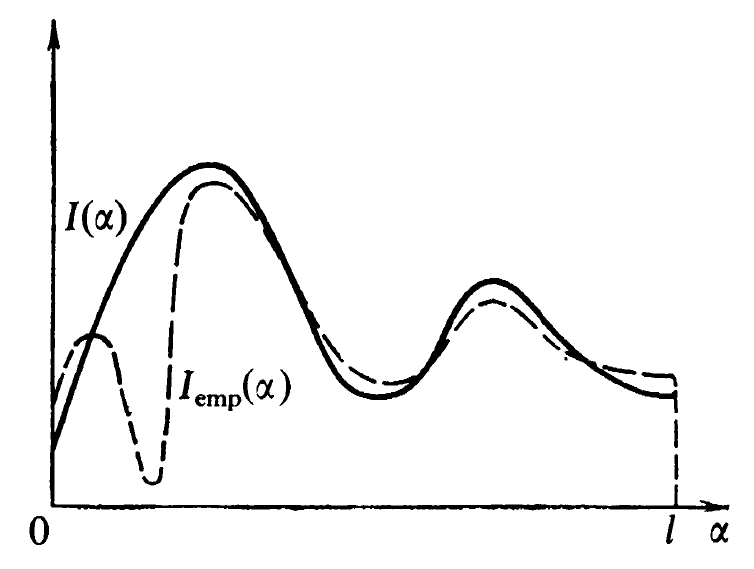
\includegraphics[width=.5\linewidth]{Imgs/frequency.png}
\caption{一致收敛示意图}
\label{fig:frequency}
\end{figure}
\begin{enumerate}
\item 依大数定律下列Hoffding不等式成立:
\begin{align}\label{ch6.15}
P\left\{\left|P\left(\alpha_{i}\right)-v\left(\alpha_{i}\right)\right|>\varkappa\right\}<2 \exp \left\{-2 \varkappa^{2} l\right\}.
\end{align}
\item 一致收敛要求
\begin{align*}
\left|P\left(\alpha_{i}\right)-v\left(\alpha_{i}\right)\right| \leq \varkappa, \quad i=1,2, \ldots, N.
\end{align*}
\end{enumerate}
\end{frame}

\begin{frame}{}
\begin{enumerate}
\item 根据一致收敛
\begin{align*}
P\left\{\sup _{i}\left|P\left(\alpha_{i}\right)-v\left(\alpha_{i}\right)\right|>\varkappa\right\} \leq \sum_{i=1}^{N} P\left\{\left|P\left(\alpha_{i}\right)-v\left(\alpha_{i}\right)\right|>\varkappa\right\}.
\end{align*}
\item 对于给定的 $N, l$和$\eta$, 我们就得到了在给定条件下的诸事件的类中, 诸频率与其概率的最大偏差的估计量就是
\begin{align}\label{ch6.19}
\varkappa=\sqrt{\frac{\ln N-\ln (\eta / 2)}{2 l}}.
\end{align}
\item 如果我们解出$l$, 那么我们就可以断言(assert), 至少以概率 (with probability) $1-\eta$ 在这个函数类上频率和概率的最大偏差不会超过$\varkappa$的样本的大小是:
\begin{align}\label{ch6.20}
l=\frac{\ln N-\ln (\eta / 2)}{2 \varkappa^{2}}.
\end{align}
\end{enumerate}
\end{frame}

\begin{frame}
\begin{solu}
对于所有的决策规则(包括那些能实现最小化经验风险的规则), 以概率(with probability) $1-\eta$
\begin{align*}
P\left(\alpha_{i}\right) \leq v\left(\alpha_{i}\right)+\sqrt{\frac{\ln N-\ln (\eta / 2)}{2 l}}
\end{align*}
使得上面的不等式同时有效.
\end{solu}
\begin{solu}
推广至无穷函数, 以概率 (with probability) $1- \eta$, 对于所有函数列不等关系
\begin{align*}
P(\alpha) \leq v\left(\alpha_{\text {emp }}\right) + 2 \frac{h\left(\ln \frac{2 l}{h}+1\right)-\ln \frac{\eta}{12}}{l}\left(1+\sqrt{1+\frac{v(\alpha) l}{h\left(\ln \frac{2 l}{h}+1\right)-\ln \frac{\eta}{12}}}\right)
\end{align*}
同时成立.
\end{solu}
\begin{solu}
一致收敛的要求不仅仅与最小化经验泛函$v(\alpha_{i})$有关, 还与决策规则的品质——即置信区间$\sqrt{\frac{\ln N-\ln (\eta / 2)}{2 l}}$——有关.
\end{solu}
\begin{solu}
\begin{enumerate}
\item 神经网络只考虑将$v(\alpha_{i})$降低, 不考虑后面的“容量控制”
\item SVMs考虑既要将$v(\alpha_{i})$降低, 同时也控制容量.
\end{enumerate}
\end{solu}
\end{frame}

\begin{frame}{3.3 必须的提示: 依概率与以概率的区别}
\begin{enumerate}
\item 随机变量序列$\xi_{1},\ldots, \xi_{l}, \ldots$依概率 (in probability)收敛至随机变量$\xi_{0}$, 即
\begin{align*}
\lim _{l \rightarrow \infty} P\left\{\left|\xi_{l}-\xi_{0}\right|<\varepsilon\right\}=1.
\end{align*}
\item 随机变量序列$\xi_{1},\ldots, \xi_{l}, \ldots$以概率 (with probability) 1收敛至随机变量$\xi_{0}$, 即
\begin{align*}
\lim _{l \rightarrow \infty} P\left\{\sup _{i \geq l}\left|\xi_{i}-\xi_{0}\right|<\varepsilon\right\}=1.
\end{align*}
\item 依概率(in probability)收敛是一种“弱的”收敛, 其根本不能保证对于每个具体实现在常规意义上的收敛性. 因此说来, 这种意义上的结论都是一种应诺(assure). 
\item 以概率(with probability)收敛是一种强收敛, 其能够保证对于每个具体实现在常规意义上的收敛性.因此说来, 这种意义上的结论都是一种断言(assert). 
\item 对于“应诺(assure)”和“断言(assert)”的区别, 完全可以理解为在战斗发起时“\textsf{给}我上”和“\textsf{跟}我上”两条命令语言背后的本质区别. 一句话, 当应诺在此岸和彼岸画上一条无法逾越的鸿沟之际, 断言则直接指认着此岸和彼岸行动的统一.
\end{enumerate}
\end{frame}



\section{第四章 统计学习理论不是统计学}
\begin{frame}{4.1 统计学习理论不可被忽略的历史}
\begin{enumerate}
\item 1962-1964年期间Vapnik和Chervonenkis在苏联控制科学院的时候他们提出广义肖像法来处理模式识别问题.
\item 我们不要粗陋的认为这种在上个世纪60年代开发出来的产品就没有意义了, 也没有必要费尽全部的力气认为只有最近出现的比较新的东西就一定是前沿的. \textbf{思想的事业从来都不以物理时间为尺度.} 这个在上世纪60年代开发出来的工具, 从1968年至今仍然是位于乌兹别克斯坦(上世纪属于苏联)境内世界上最大的露天金矿——穆伦陶(Murun-Tau)——运行的唯一找矿系统. Chervonenkis也因在穆伦陶金矿上的成功而获得1987年苏联最高奖: 苏联国家奖. 值得提及的是在Chervonenkis去往穆伦陶之前, 该矿所用的找矿系统是拉丁方方法.
\item 那时苏联控制科学院没有\textbf{数字计算机}, 仅有的是\textbf{模拟计算机}. 这样一来在输入初始化数据就带来很大的困难, 他们是通过手工或者借助计算器计算内积的, 然后再将内积借助可调节的电阻信号输入模拟计算机. Vapnik和Chervonenkis自一开始就没有针对经验数据直接地进行操作(而统计学总是对经验数据直接地进行操作). 后来到了1964年, 苏联控制科学院有数字计算机后广义肖像法就部署在数字计算机上用来解决各类模式识别问题
\end{enumerate}
\end{frame}

\begin{frame}{4.1 统计学习理论不可被忽略的历史}
\begin{enumerate}
\item 对于可分情况下其目标是最大化下列泛函(这一步非常重要, 这就是对诸函数的类(the class of functions)的控制, 而不是对诸函数的控制. 诸函数不需要我们控制, 也不需要我们假设. 诸函数就是由机器实施的\{0,1\})
\begin{align}
\label{max-functional}
\rho_0  = \min_{\{i:y_i = 1\}}[(\frac{w}{|w|},x_i)+b] - \max_{\{j:y_j = -1\}}[(\frac{w}{|w|},x_j)+b]
\end{align}
其约束条件是
\begin{align}\label{after2.3}
y_i((w,x_i)+b) \geq 1, i=1,\ldots,l.
\end{align}
\item 这一问题的等同于在线性约束下求解二次型最小值问题
\begin{align*}
R_1(w,b) = (w,w).
\end{align*}
设最小值在 $w=w_0$ 处取得, 则
\begin{align*}
\rho_0 = \frac{2}{\sqrt{(w_0,w_0)}}.
\end{align*}
\end{enumerate}
\end{frame}

\begin{frame}{4.1 统计学习理论不可被忽略的历史}
关于最优分隔平面的陈述是再熟悉不过的了, 但我们如何本质地阐说这一问题呢? 让我们先把内积 $(x_{i}, x_{j})$ 写成矩阵的形式. 对于经验观测数据
\begin{equation}
X_{l \times d} = \begin{bmatrix}
x_{11} & x_{12} & \ldots & x_{1d}\\
x_{21} & x_{22} & \ldots & x_{2d} \\
\vdots & \vdots & \ddots & \vdots \\
x_{l1} & x_{l2} & \ldots & x_{ld}
\end{bmatrix},
\end{equation}
那么内积矩阵就可以写成\textsf{关于经验数据$X$自身$X=(x_{1}, x_{2}, \ldots, x_{l})$的线性组合的形式},
\begin{equation}
XX^{T}_{l \times l} = \begin{bmatrix}
\ldots & \ldots & x_{1} & \ldots & \ldots\\
\ldots & \ldots & x_{2} & \ldots & \ldots \\
	   &        & \vdots &  &  \\
\ldots & \ldots & x_{l} & \ldots & \ldots
\end{bmatrix}
\begin{bmatrix}
\vdots & \vdots &   & \vdots\\
\vdots & \vdots &   & \vdots \\
x_{1}  & x_{2}  & \ldots  & x_{l} \\
\vdots & \vdots &   & \vdots \\
\vdots & \vdots &   & \vdots
\end{bmatrix}
= \begin{bmatrix}
[X][x_{1}], & [X][x_{2}], &  \ldots, & [X][x_{l}]
\end{bmatrix}.
\end{equation}
\end{frame}

\begin{frame}{4.1 统计学习理论不可被忽略的历史}
\begin{enumerate}
\item 对内积这样的分析即将意味着什么呢? 如果我们还没有忘记\textit{Grundbegriffe}中关于概率论如何本质地区别于测度论, 那么现在来看当我们将经验数据视为独立随机变量之后, 以上“观测样本$x_{1}, \ldots, x_{l}$作为数学空间的‘正交基函数’”就显得是那么的容易理解. 
\item 的确, 对于消化了Kolmogorov概率论的Vapnik和Chervonenkis来说这并不是什么值的额外拿出来言说的. 
\item 然而, 由于统计学家们仅仅是将概率看成处理噪音的工具, 因此他们绝对不会在Kolmogorov概率论意义下思考问题. 但是对于接受统计学教育的我们需要对此做出一些说明.  因为只有当经验数据被视为随机变量的时候, 内积就可以理解为数据自己作为正交函数来构建数学空间, 然后将经验数据投影在此数学空间上, 这就使得我们处理的问题直接进入泛函分析的领域而不再是知性科学. 
\item 问题不在于对坐标(coordinates)的求解——统计学就始终在求解坐标(coordinates)的系数, 而在于求解正交函数的系数(coefficients). 
\item 因此, 我们无论如何都不能用理解统计学的思想来理解SVMs. 如果按照统计学理解方式, 那么对于手写数字我们就应该挑选某一个像素坐标; 但是对于SVMs而言, 数据的排列方式对我们影响不大——甚至可以随机化像素也不会对预测精度产生影响(Bottou 1994)——我们只要关注内积即可, 关注内积实际上就是直接进入泛函分析 (Vapnik, 2006, p.447).
\end{enumerate}
\end{frame}

\begin{frame}{4.1 统计学习理论不可被忽略的历史}
\begin{solu}
如果我们在二阶多项式空间构建SVMs, 那么我们要创建的特征空间$Z$就一共要有 $N = \frac{n(n+3)}{2}$个坐标, 即
\begin{align*}
z^{1} = x^{1}, \ldots, z^{n} = x^{n}, \\
z^{n+1} = (x^{1})^{2}, \ldots, z^{2n} = (x^{n})^{2}, \\
z^{2n+1} = x^{1}x^{2}, \ldots, z^{N} = x^{n}x^{n-1}.
\end{align*}
\end{solu}
\begin{solu}
那么我们需要这样\textbf{显式地}构建特征空间吗? 答案是{\color{red}{否定的}}. 根据Hilbert-Schmidt理论, 在Hilbert空间的内积有等同的表示:
\begin{align*}
(z_{1} * z_{2}) = \sum_{r=1}^{\infty}a_{r}z_{r}(x_{1})z_{r}(x_{2}) \Longleftrightarrow K(x_{1}, x_{2}), a_{r} \geq 0.
\end{align*}
\end{solu}
\begin{enumerate}
\item 采用核方
法的创举最后被统计学家们称为是“Kernel trick”(核计俩) (Hastie et al., 2009, p.
624, p. 660), (Efron et al., 2016, p. 375). 而也正是因为统计学家根本不懂何为真正的数学空间, 所以他们就很难理解为什么SVMs 要构建无限维数学空间——构建的方法是核方法. 他们是这样说的(James et al., 2017, p. 383):
\end{enumerate}
\end{frame}

\begin{frame}{4.1 统计学习理论不可被忽略的历史}
\begin{solu}
虽然他们这一章对SVMs 的陈述全部都是彻底的错误, 但是为了说明白他们的彻底错误, 我们就不得不再翻出来引用几句(James et al., 2017, p. 383):
\end{solu}
\begin{enumerate}
\item “因为在很多SVMs的应用领域, 那扩充后的特征空间是如此那般的大以至于其计算是相当棘手的. 对于许多核函数, 例如径向基核函数 (9.24)(表达式(9.24)的表述是错误的, 因为他们是针对坐标来求核函数的, 但这并不影响他们这些统计学大师们继续再全部错下去.), 它的特征空间是\textbf{隐式的}并且是无限维数的, 所以无论如何我们永远都无法在那里进行计算!” (“!”是统计学家自己加的, 这个“!”除了反映北美统计学的无头脑外, 再没别的作用)
\item “核方法中隐含的二次惩罚意味着对将所有特征都包含在模型中,因此稀疏性通常不是一种选择。 为什么会有这种肆无忌惮的热情? ” (Efron et al., 2016, p. 387)
\end{enumerate}
\end{frame}

\begin{frame}{4.1 统计学习理论不可被忽略的历史}
\begin{enumerate}
\item 这就是当今\textsf{统计学绝对的英雄们}自己捧出他们的基于统计学来理解的SVMs. 并不需要太多的聪明就可以看出, 在这种对SVMs的曲解中, 正是知性科学和无头脑掌控了整个局面; 同样不需要太多的聪明就可以看出, 这种局限在知性科学的学术, 事实上是以更加一般的无头脑——即没有任何思想——作为基础支柱的. 这些统计学大师并且包括大师的得意门生在内的无头脑只不过反映出北美统计学——亦即当下全部统计学——绝对的贫困. 
\item 有一群好汉一天忽然想到, 数据之所以表现不好, 是因为他们被那些观测变量组成的函数给迷住了. 如果他们换一种方式抛掉那烦人的函数, 比方说用精心挑选的另外的几个变量来重新组合一下, 那么他们就会避免任何数据失效的危险. 这样的一群好汉一辈子都在同这样的函数作斗争, 统计学的方法给他们提供了愈来愈多的有关这种函数可改进的证明. 这样的一群好汉正就是当下整个统计学家们的标本.
\end{enumerate}
\end{frame}

\begin{frame}{4.1 统计学习理论不可被忽略的历史}
\begin{enumerate}
\item 这些统计学大师们将数学空间视为朴素的、由经验观测变量直接构成的对象, “无限维数的特征空间”也因此在他们看来是无法理解的, 因此也就无法直接经验地计算. 确实, 当我们把知识的理解仅仅交给知性科学下的统计学, 把知识仅仅变成跟在统计学后面的亦步亦趋, 那么我们是怎么都不可能进入Hilbert、Kolmogorov等思想家的事业, 我们就一定会如同这些统计学家们一样, 将SVMs仅仅安置在统计学教科书的某个中间章节. 这样的成果越是大面积的出现, 就越证明着对Vapnik思想理解的遥远, 同时也越是指认着对Vapnik思想真正阐述的必然的需要——如果我们还承认自己在从事那激动人心的科学的事业的话.
\item 所以, 我们就从根本上看到无论是从问题的提出还是问题的解决方案, 统计学习理论都与统计学截然不同, 并且这种不同根本不局限在技术层面, 而直接是整个哲学根基的不同. 哲学给予思想的真正馈赠不仅仅是结论而更应该是批判的方法. 唯有通过这种方法我们才有可能摆脱黑格尔所谓的“门外汉”; 唯有通过这种方法我们才有可能将Vapnik给出的“不要再错下去”的谆谆教导积极地开启出来, 从而那关于学习问题的现实内容本身——即何谓知识的本质——方才有可能同我们真正照面. 因此, 也正是在这个意义上我们坚决断言: 
\begin{center}
{\color{red}{统计学习理论不是统计学.}}
\end{center}
\end{enumerate}
\end{frame}

\begin{frame}{4.2 现象学的学习理论}
\begin{solu}
这样一来, 我们就根本无法再通过理解统计学的思维方式、基于统计学的哲学来理解、阐述统计学习理论. 当然至于统计学到底发生了什么以及到底还能有可能发生什么, 那只有统计学家们自己最清楚. 对我们而言针对统计学的言辞批判到此结束, 余下的唯有快快立刻行动!
\end{solu}
\begin{solu}
\begin{enumerate}
\item Hilbert于1938年发表的著作《\textit{Grundz\"{u}ge der Theoretischen Logik}》(Principles of Mathematical Logic)中找到. 这部著作根本性地为整个20世纪数学的根基——即数学是纯粹理性的产物——标定了基本的路标. 按照Hilbert的原则, 纯粹数学逻辑的原则被这样定义(Hilbert et al., 1950, p. 5):

\begin{quotation}
{\ttfamily
“
... 最终, 以下的一般陈述是非常重要的. 根据我们对诸基础逻辑连接词的定义, \textsf{一句语句组合的正确或错误单独地依赖于输入语句的那组合本身的正确或者错误, 而并不依赖于输入语句的内容.}
”
}
\end{quotation}
\item Hilbert 的陈述是针对数学逻辑的, 这是在本体论层面给出的基础. 当数学逻辑从纯粹输入命题组合的正确-错误出发而不关心任何内容时, 它逻辑地预设了主客
体之间的分立.  问题的核心在于“独立”.
\end{enumerate}
\end{solu}
\end{frame}

\begin{frame}{4.2 现象学的学习理论}
\begin{enumerate}
\item Kolmogorov 没有就概率论中的核心概念——独立——的哲学根基展开阐述,
他聚焦在以独立为基础的逻辑上展开概率论的阐述. 但是对于今天的我们而言,
我们确实需要批判地看待独立. 这样一来就我自己知识而言我们就不得不借助
Bruno de Finetti 的启发来加以进一步地阐述. 
\item Bruno de Finetti (1975) 在阐述他的观点时提出了“概率本不存在”的概括. 也就是说我们在不需要假设独立的前提下仍然是可以完成概率论的建构, 而此时对应的概念是他提出的“可交换”(exchangeability) (Bruno de Finetti, 1975, p. 434 ). 
\item 因为当经验观测被视为独立随机变量的时候, 很明显此时独立随机变量作为基函数构建数学空间——虽然按照数学传统此空间被称为“Hilbert 空间”, 但是如果我们严格说来, 这样的空间称作“Kolmogorov 空间”在哲学的理解上更为严谨——就完全等同于正交函数所构建的数学空间.
\end{enumerate}
\end{frame}

\begin{frame}{4.2 现象学的学习理论}
\begin{enumerate}
\item 然而, 当数字计算机出现后这种“假设经验数据满足相互独立”的要求其
实是已经被扬弃了的——并且也正是因为做到了扬弃才有我们后面要介绍的
研究内容——这一点我们来看核函数就完全能够理解
\item Vapnik对于核函数与级数之间的批判关系也是知晓的, 我们以RBF核函数为例来说明这一问题 (Vapni, 2019). 
\item 在近似理论中扮演重要角色的是埃尔米特(Hermit)多项式和埃尔米特函数. 埃尔米特多项式$H_{1}(x),\ldots,H_{k}(x),\ldots$定义了基于权重$\exp\{-x^{2}\}$的正交多项式, 也就是说,
\begin{align*}
\int_{-\infty}^{\infty} P_{s}(x)P_{n}(x)e^{-x^{2}}dx = 2^{n}n!\sqrt{\pi}\delta_{n,s},
\end{align*}
其中, 这里$\delta_{n,s}$是克罗内克(Kronecker)符号(如果$s \neq n$, $\delta_{s,n} = 0$, 如果$s=n$, $\delta_{s,n} = 1$).
\item 下列正交基函数
\begin{align*}
e_{n}(x) = (2^{n}n!\sqrt{\pi})^{-1/2}H_{n}(x)e^{-\frac{x^{2}}{2}}
\end{align*}
被称作是埃尔米特函数.
\end{enumerate}
\end{frame}

\begin{frame}
\begin{enumerate}
\item 1866年, Mehler证明, 对于任意的$0 < \varepsilon < 1$, 下列等式成立
\begin{align*}
K_{M}(x,x^{\prime}) = \sum_{k=0}^{\infty}\varepsilon^{k}e_{k}(x)e_{k}(x^{\prime}) = \frac{1}{\sqrt{1-\varepsilon^{2}}}\exp \left\{ -\frac{\varepsilon^{2}(x-x^{\prime})^{2} + 2(\varphi - \varepsilon^{2})xx^{\prime}}{1-\varepsilon^{2}} \right\}.
\end{align*}
此等式的右侧项叫做\textsf{Mehler核}. 
\item 标准化的Mehler核就是RBF核, 即
\begin{align*}
K(x,x^{\prime}) = \frac{K_{M}(X,X^{\prime})}{\sqrt{K_{M}(x,x)K_{M}(x^{\prime},x^{\prime})}} = \exp\{\delta(x-x^{\prime})^{2}\}
\end{align*}
其中, 这里的参数$\delta > 0$是被下列值$\varepsilon$定义的
\begin{align*}
\delta = \frac{\varepsilon^{2}}{1-\varepsilon^{2}}.
\end{align*}
\item 我们这里强调的是, Mehler核需要前提: 必须首先要在独立正交函数的基础上才能进展; 但是计算机出现后利用RBF就不需要独立, 而是“让数据彼此打交道”. 这在存在论(ontology)上是完全不一样的哲学理念. 这就是{\color{red}{现象学还原的方法对先前的理论做扬弃}}.
\end{enumerate}
\end{frame}

\begin{frame}{4.2 现象学的学习理论}
\begin{enumerate}
\item 然而, 这些都还不是模式识别问题最优越的特征. Vapnik的老师Lerner给出了他对于模式识别问题本质的理解. (Lerner, 1972):

\begin{quotation}
“模式识别问题的独特之处在于相信这样的一个事实, 即所要求解
的\textbf{诸规则的类}(the class of functions)是极其简单的. 最好使用\textbf{诸决策函数的类}来找到风险最
小化问题中那最独特的特征....”
\end{quotation}
\item 控制的不是“诸函数”而是“诸函数的类”. “诸函数”不需要控制
%它们只不过是由计算机内部逻辑电路的开合实现的{0,1}示性函数.
%\item Bruno de Finetti (1975) 诚实地在自己的著作中表达了影响自己思想的哲学是休谟. 
%\item 我们也不得不在这里诚实地表达——这是不得不说出来的——为了能进一
%步阐说, 我的思想的确就是受到马克思哲学的影响. 
%\item 马克思在《哲学的贫困》中给出“使用价值”和“交换价值”的区分. 
%\item 受此启发, 当我们把理解统计学习理论问题从哲学的层面加以审视的话, 我们不难发现, 只有当我们将这里的内积看成数据的真正的具体“社会活动”的时候, “生产”的概念才能真正同我们照面. 而此时“交换”的概念就如其所是地向我们呈现. 
%\item “生产”就是对“独立”的扬弃. 在生产的概念中, 活动的主体性原则得以保留而抛弃了抽象的独立要求.
\end{enumerate}
\end{frame}


\begin{frame}{4.2 现象学的学习理论}
\begin{enumerate}
\item 当我们以生产的视角来审视SVMs时, 我们就更有语言的底气来展开后续的阐说. 我们知道, 最大化间隔 (\ref{max-functional}) 的解 $w_{0}$和$b_{0}$必须满足KKT条件
\begin{align}
\label{kkt}
\alpha_{i}^{0}(y_{i}((x_{i}, w_{0}) + b_{0}) - 1) = 0, i = 1, \ldots, l.
\end{align}
从KKT条件我们知道, 仅仅是取值非零的$\alpha_{i}^{0}$所对应的那些向量$x_{i}$才使得所求的分隔超平面成立
\begin{align}
\label{kkt-hyperplane}
y_{i}((x_{i}, w_{0}) + b_{0}) = 1.
\end{align}
这一点对于熟悉SVMs的读者来说一点都不陌生. 那么也就是说, 当我们控制诸函数的类(the class of functions)之后, 我们得到了这样的结果: 
\item 通过控制诸函数的类, 由\textbf{所有样本}生产出来的\textbf{若干支持向量}才使得机器具有学习能力. 而\textbf{少数的支持向量}就是由全体样本的“社会活动”通过优化得到的.
\end{enumerate}
\end{frame}

\begin{frame}{4.2 现象学的学习理论}
\begin{figure}
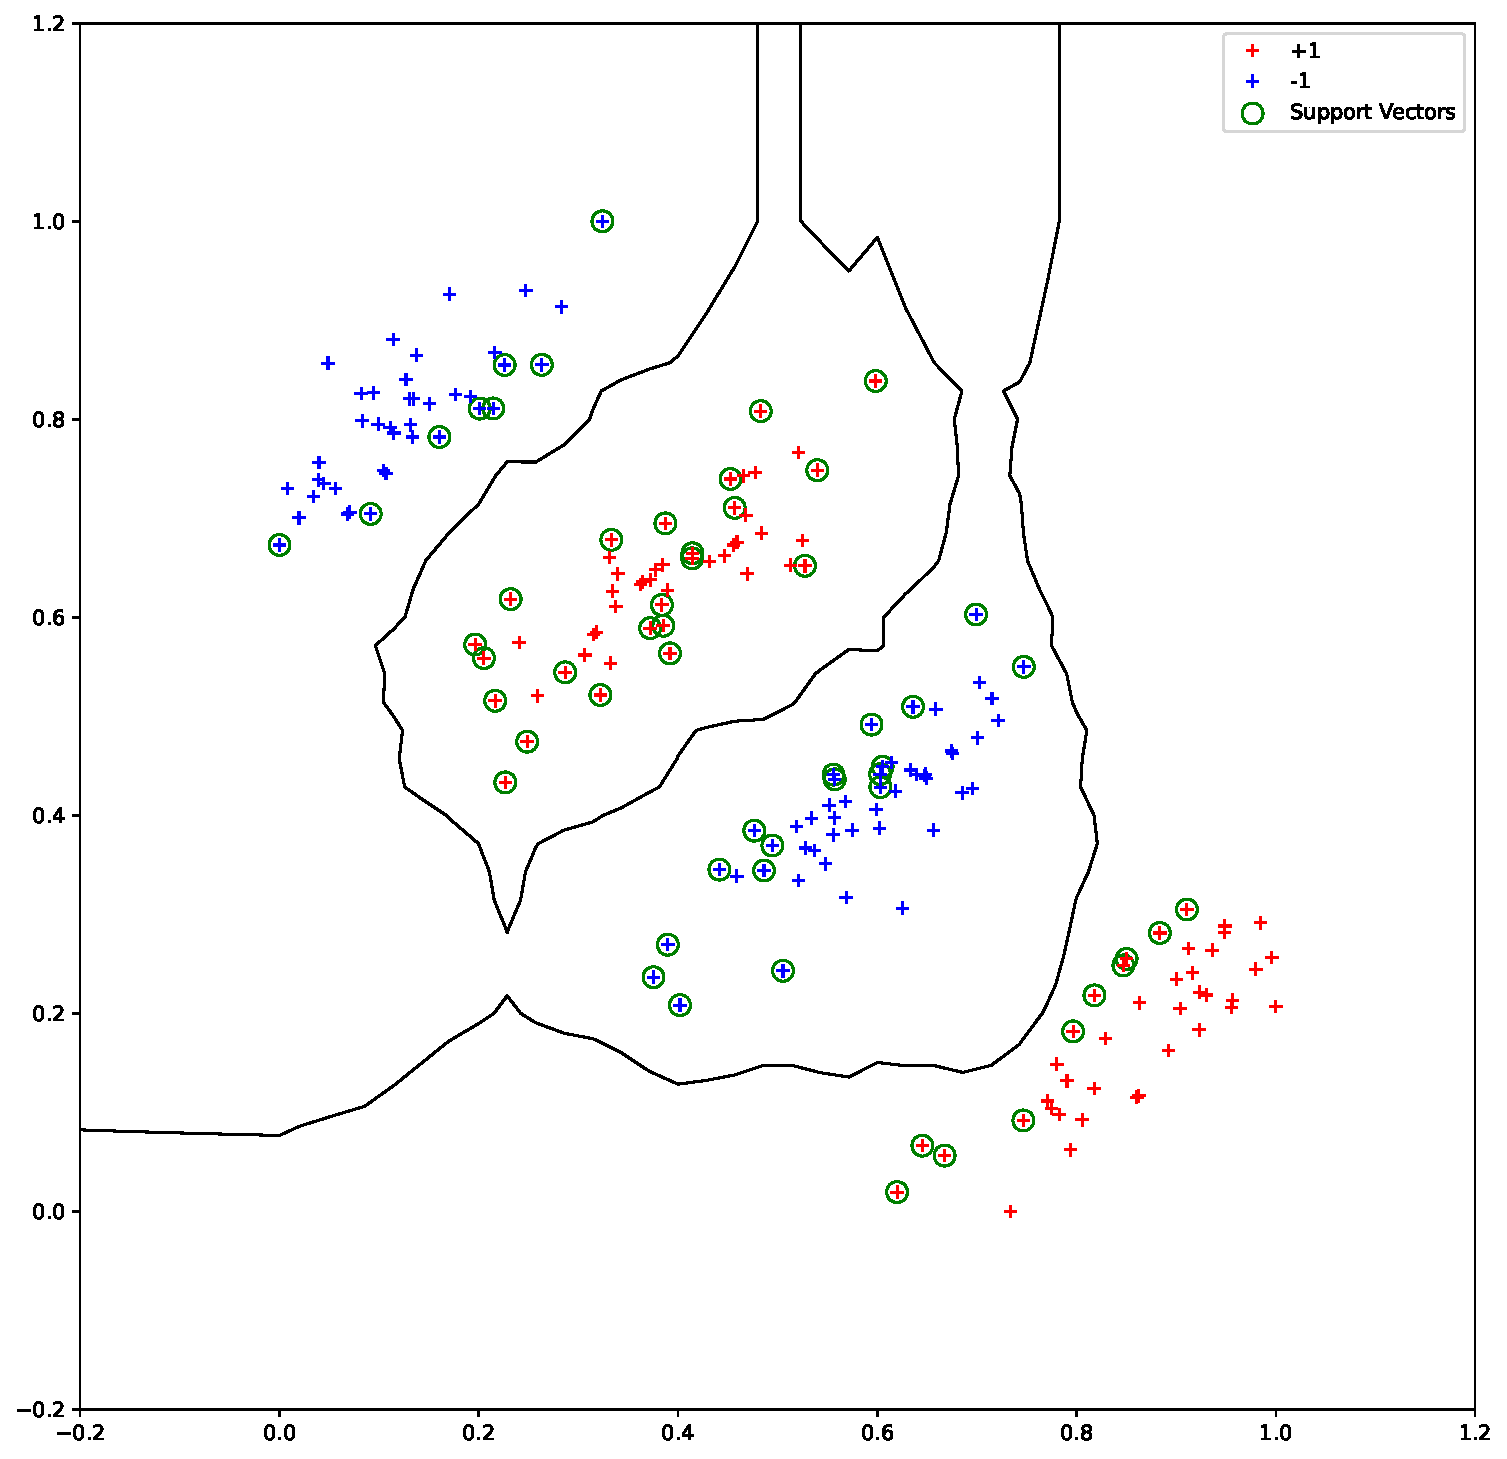
\includegraphics[width=.45\linewidth]{Imgs/svm-ink0.pdf}
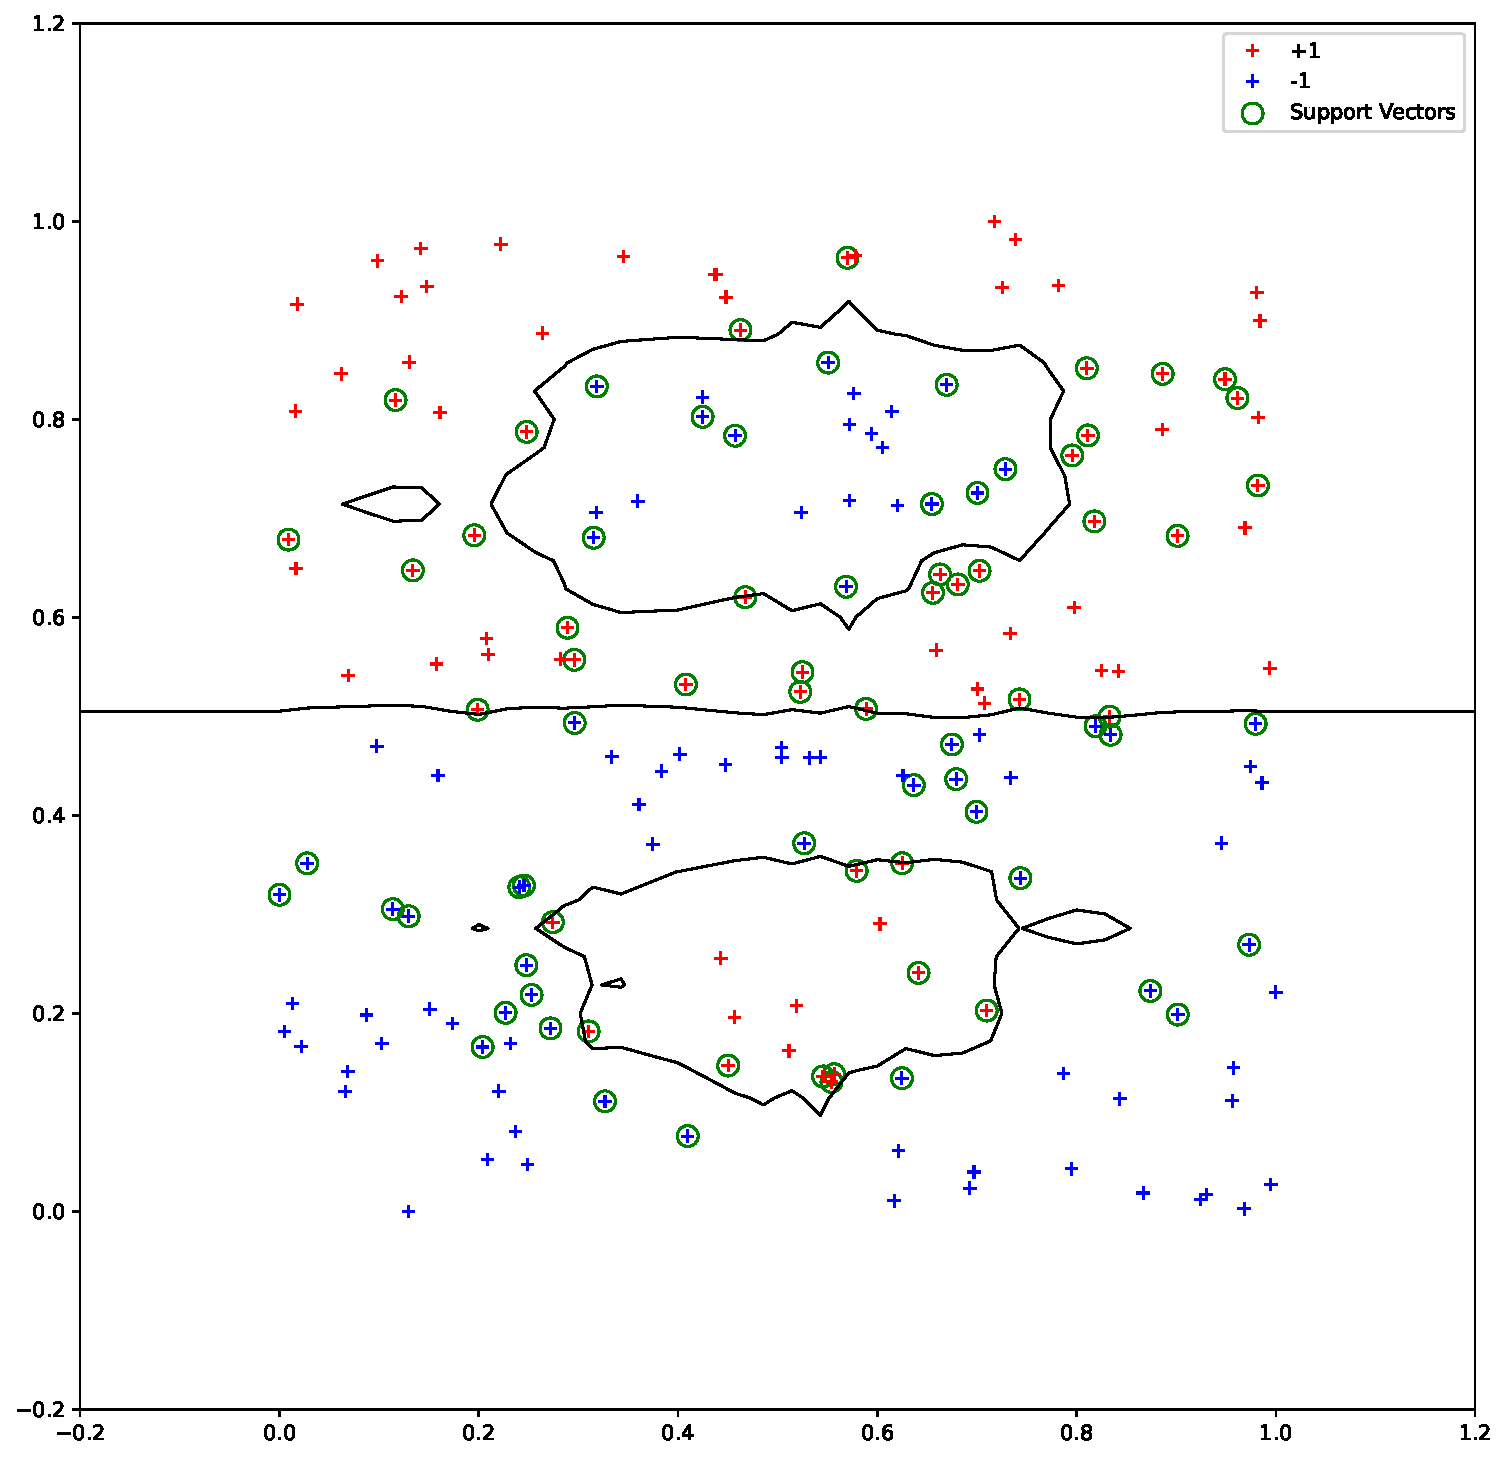
\includegraphics[width=.45\linewidth]{Imgs/svm-xoxo.pdf}
\captionsetup{labelformat=empty}
\caption{支持向量演示}
\end{figure}
\end{frame}

\begin{frame}{4.2 现象学的学习理论}
\begin{enumerate} 
\item 通过控制诸函数的类, 由\textbf{所有样本}生产出来的\textbf{若干支持向量}才使得机器具有学习能力. 而\textbf{少数的支持向量}就是由全体样本的“社会活动”通过优化得到的.
\item 受启发于现象学还原, 我们这里可以看到, 只有计算得到的非零的$\alpha_{i}$——即支持向量——才会对那类似规律(即知识)有作用. 非支持向量不会产生作用. 这就是“异化”. 即由“所有样本”生产出来的“支持向量样本”反而支配、控制大多数样本.
\item 正是在这个意义上, Vapnik和Chervonenkis才说SVMs是“暴力算法”. “暴力”的所指就是对$\alpha$的深刻理解上. 这一点无论是Vapnik、Chervonenkis还是Vovk都是深知的.
\end{enumerate}
\end{frame}


\section{第五章 可信机器学习——Conformal Prediction方法}
\begin{frame}
\begin{figure}
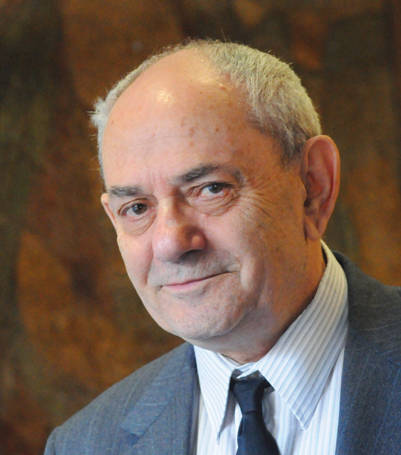
\includegraphics[width=.3\linewidth]{Imgs/vapnik-copa.jpg}
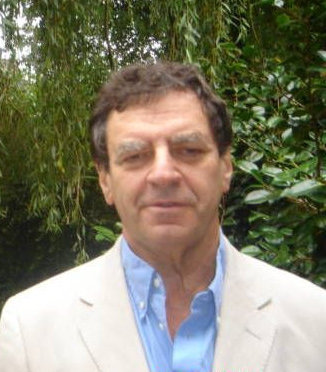
\includegraphics[width=.3\linewidth]{Imgs/alex2.jpg}
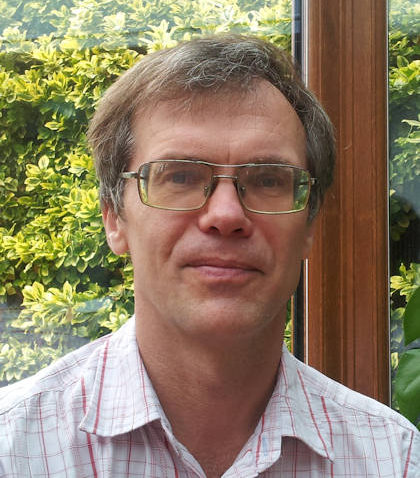
\includegraphics[width=.3\linewidth]{Imgs/volodya.jpg}
\captionsetup{labelformat=empty}
\caption{Vladimir N. Vapnik \quad Alexander Gammerman \quad Vladimir Vovk}
\end{figure}
\end{frame}

\begin{frame}{5.1 Conformal Prediction}
\begin{enumerate}
\item 机器学习的输出是“暴力得分”, 可信机器学习需要对暴力得分校正.
\item 我们不仅仅得到“暴力”的单个预测, 还可以“软化”成“集合预测”.
\end{enumerate}

\begin{table}[]
\centering
\caption{SVMs-CP方法的对于高超声速飞行器不确定度量结果}
\label{tab:cp-svm}
\begin{tabular}{@{}ccccccc@{}}
\toprule
\#  & -1        & 1        & 真实标签 & SVMs-CP标签 & 置信度 & 可信度 \\ \midrule
0	&0.872483	&0.613115	&-1	&-1	&0.386885	&0.872483\\
1	&0.845638	&0.619672	&-1	&-1	&0.380328	&0.845638\\
2	&0.184564	&0.960656	&1	&1	&0.815436	&0.960656\\
3	&0.825503	&0.655738	&-1	&-1	&0.344262	&0.825503\\
4	&0.755034	&0.718033	&-1	&-1	&0.281967	&0.755034\\
5	&0.446309	&0.849180	&1	&1	&0.553691	&0.849180\\
11	&0.718121	&0.721311	&-1	&1	&0.281879	&0.721311\\
12	&0.718121	&0.721311	&-1	&1	&0.281879	&0.721311\\
\bottomrule
\multicolumn{1}{l}{} & \multicolumn{1}{l}{} & \multicolumn{1}{l}{} & \multicolumn{1}{l}{} & \multicolumn{1}{l}{} & \multicolumn{1}{l}{} & \multicolumn{1}{l}{}
\end{tabular}
\end{table}
\end{frame}

\begin{frame}{5.1 Conformal Prediction}
\begin{enumerate}
\item 机器学习的输出是“暴力得分”, 可信机器学习需要对暴力得分校正.
\item 我们不仅仅得到“暴力”的单个预测, 还可以“软化”成“集合预测”.
\end{enumerate}

\begin{table}[htbp]
\renewcommand{\arraystretch}{1.3}
\caption{高超声速飞行器的集合预测结果}
\label{tab:set-prediction}
\centering
\begin{tabular}{lrrllllllr}
\toprule
{} &         0 &         1 &     .0 & .01 & .05 &  .2 &  .5 & .95 &  真实标签 \\
\midrule
0 &  0.001578 &  0.490446 &  [0, 1] &  [1] &  [1] &  [1] &   [] &   [] &     1 \\
1 &  0.079073 &  0.008217 &  [0, 1] &  [0] &  [0] &   [] &   [] &   [] &     0 \\
2 &  0.821253 &  0.000954 &  [0, 1] &  [0] &  [0] &  [0] &  [0] &   [] &     0 \\
3 &  0.002549 &  0.250972 &  [0, 1] &  [1] &  [1] &  [1] &   [] &   [] &     1 \\
4 &  0.002752 &  0.387290 &  [0, 1] &  [1] &  [1] &  [1] &   [] &   [] &     1 \\
\bottomrule
\end{tabular}
\end{table}
\end{frame}

\begin{frame}{5.1 Conformal Prediction}
\begin{table}[htbp]
\caption{集群真实数据集的简单预测结果}
\label{tab:simple-prediction}
\centering
\begin{tabular}{lrrrrrr}
\toprule
{} &         0 &         1 &  真实标签 &  MCP预测标签 &     置信度 &     可信度 \\
\midrule
0 &  0.001578 &  0.490446 &     1 &    1 &  0.998422 &  0.490446 \\
1 &  0.079073 &  0.008217 &     0 &    0 &  0.991783 &  0.079073 \\
2 &  0.821253 &  0.000954 &     0 &    0 &  0.999046 &  0.821253 \\
3 &  0.002549 &  0.250972 &     1 &    1 &  0.997451 &  0.250972 \\
\bottomrule
\end{tabular}
\end{table}
\end{frame}

\begin{frame}{5.2 分布漂移检测}
\begin{enumerate}
\item 从“归纳主义科学”的立场中彻底摆脱出来;
\item 终止全部形而上学引领下的知识论路向(或范畴论路向), 并且在技术上
揭破这一路向的局限性;
\item 洞穿并全面瓦解“分布(Distributions) 是名词”这一统计学的根基.
\end{enumerate}

\begin{solu}
\begin{enumerate}
\item 统计学认为分布是由统计学家假设出来的, 他们总是假设各种分布
\item Vapnik-Chervonenkis 告诉我们, 分布是被生产出来的, 是数据最本质的内容, 并且这种生产出来的分布会否定已经学到的知识
\item 分布漂移是因为支持向量的改变造成的. 所以SVMs一定得写成复数, 而不是单数.
\item 分布是动词, 是变化, 是复数, 会随着学习的进程而发生漂移、运动
\item 随机化会使得power probability distributions消除.
\item 在处理实际具体问题的时候, 不能随机化数据, 应该诚实地按照数据本有的顺序学习.
\end{enumerate}
\end{solu}
\end{frame}

\begin{frame}{5.2 分布漂移检测}
\begin{figure}[htbp]
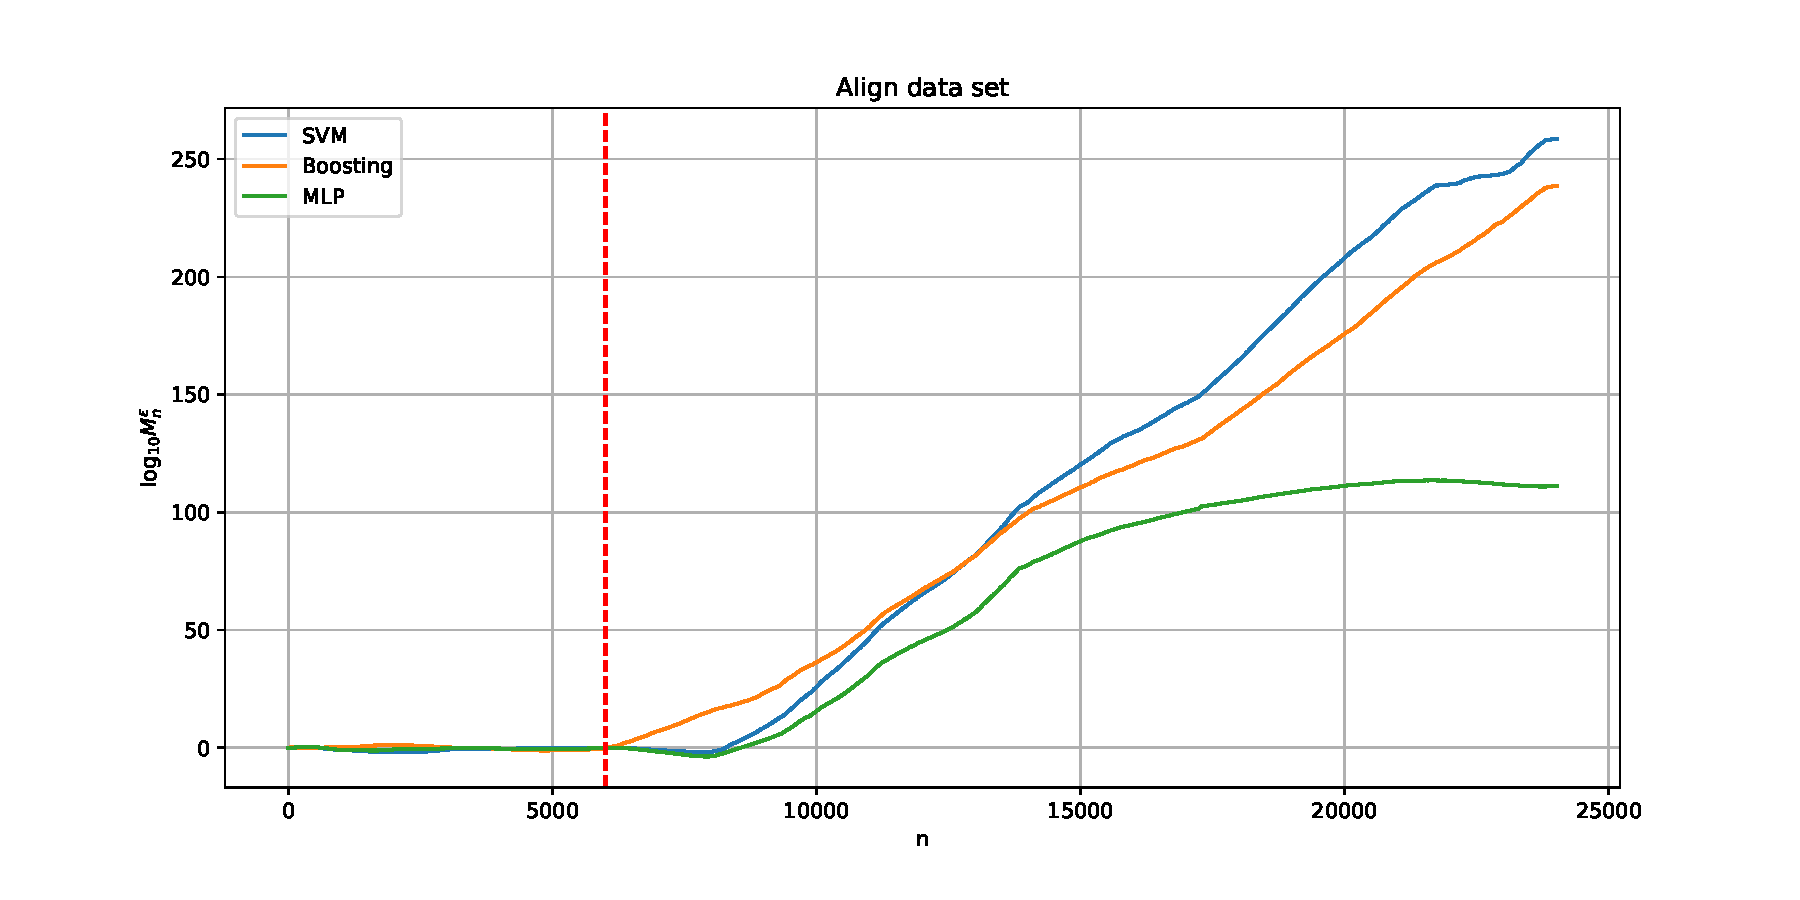
\includegraphics[width=.7\linewidth]{Imgs/Align data set-icml}
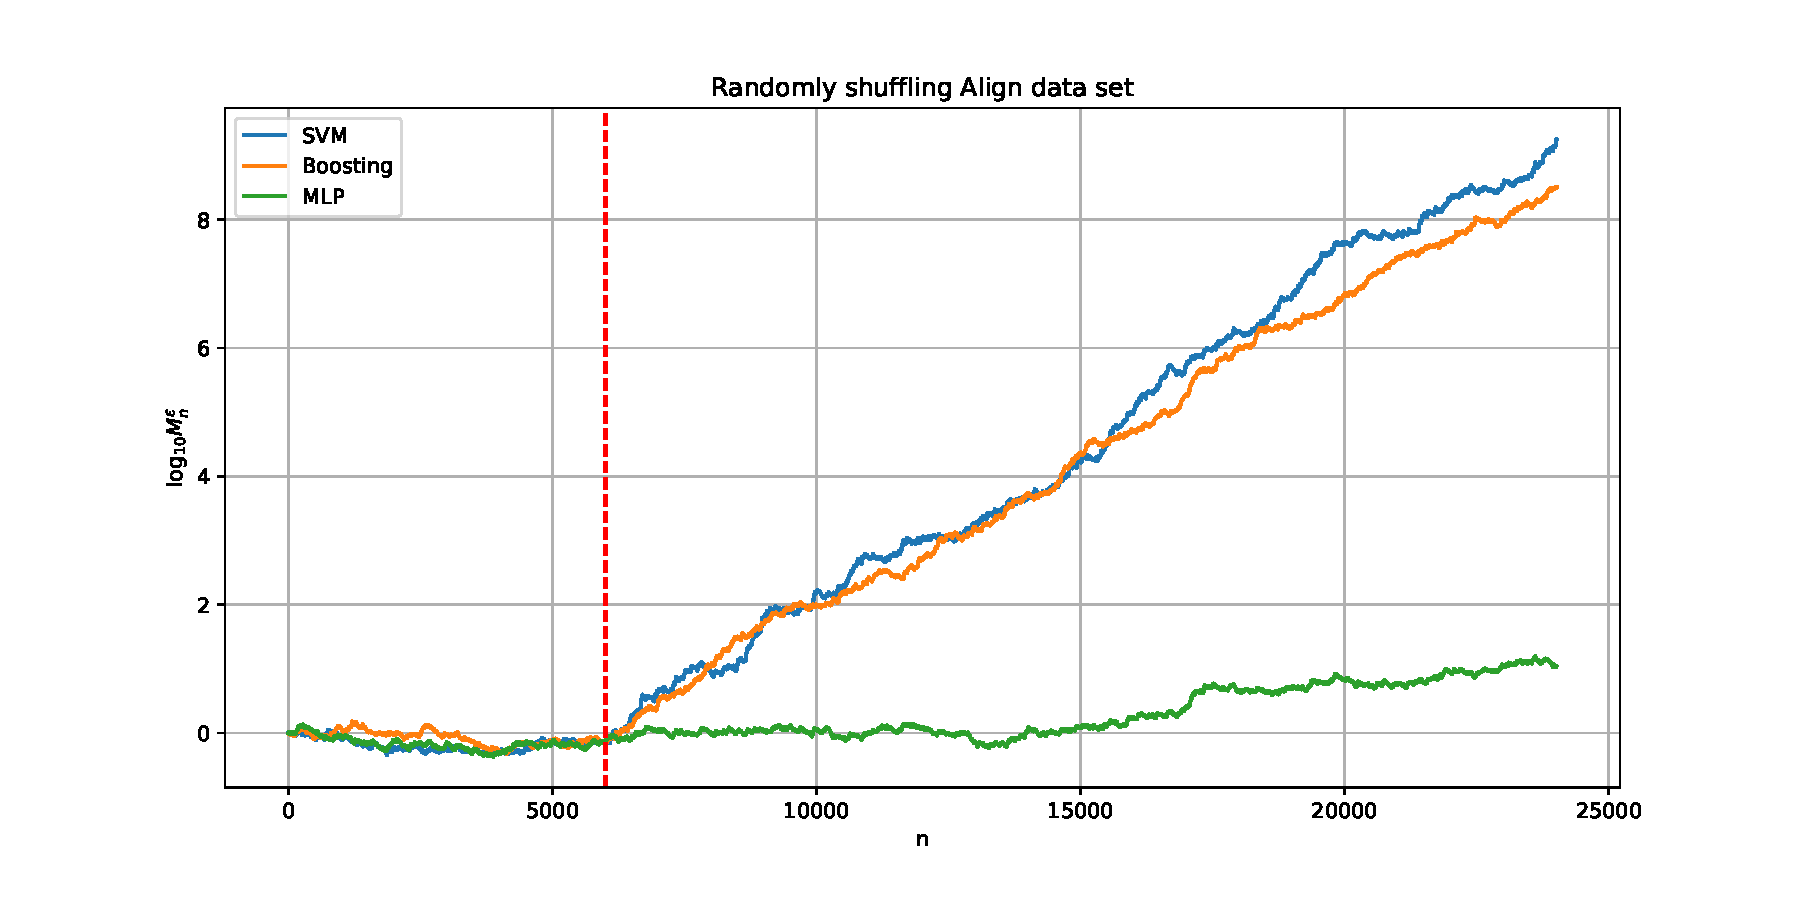
\includegraphics[width=.7\linewidth]{Imgs/Randomly shuffling Align data sett-icml}
\caption{Swarm数据随机化处理前后分布漂移检测}
\label{fig:flock-mar}
\end{figure}
\end{frame}


\section{第六章 智慧学习}
\begin{frame}{6.1 “深度学习”:思入知识本质的那一深度}
\begin{enumerate}
\item[1.] \textsf{对于可分情形:} 其一致收敛的速度的界
\begin{align*}
P(yf(x, \alpha_{l}) \leq 0) < O^{*}\left(\frac{h - \ln \eta}{l}\right)
\end{align*}
以概率 (with probability) $1-\eta$ 成立.
\item[2.] \textsf{对于不可分情形:} 其一致收敛的速度的界
\begin{align*}
P(yf(x, \alpha_{l}) \leq 0) < v(\alpha_{l}) + O^{*}\left(\sqrt{\frac{h - \ln \eta}{l}}\right)
\end{align*}
以概率 (with probability) $1-\eta$ 成立.
\end{enumerate}
\begin{solu}
经验地说, 这就表明为了获得相同阶数的收敛, 在可分情形下只要320个样本而在不可分情形下则需要10000个样本. 为什么会有这么大的差距呢? 

Vapnik的思考从来没有离开哲学半步. Vapnik为人类学习不需要太多样本的解释在于{\color{red}{“人类的学习快速是因为人类有个老师”}}.
\end{solu}
\end{frame}

\begin{frame}{6.1 “深度学习”:思入知识本质的那一深度}
\begin{enumerate}
\item 人类的这个老师并不教你知识(教知识的老师是近代的事情, 自古以来的老师都不教知识, 而都是教智慧)而是教我们智慧
\item 教给我们大局观、整体观, 教给我们直观 (所谓直观就是能说出“整体一定大于个体”这样的陈述). 
\item 这样的老师在人类知识的获取上扮演了极为重要的角色, 一句话, 老师提供给我们智慧, 而\textsf{智慧就是使用学习问题} (Intelligence is Using Learning Problems).
\item $n$-维数学空间的VC维是$n+1$.
\item 正因为VC理论告诉我们$n$-维数学空间的VC维是$n+1$, 所以我们在对知识本身做学习的时候, 就是真正的思入知识之本质的一度中去, 这就是智慧. (真正意义上的“深度学习”. “深度学习”不是把网络搞的深深的、层数搞得多多的, 而是思想的深度进入知识的本质的一度.)
\item 老师教你的大局观、整体观就是将你从知识中领出来、让你对知识本身再进行一次观照.
\item 我们要对机器的输出(这是知识)再进行学习(这是智慧).
\end{enumerate}
\end{frame}

\begin{frame}{6.2 使用统计不变量学习, 完备统计学习理论: 谓词学习}
\begin{enumerate}
\item 我们将模式识别问题定义为估计诸条件概率 $P(y = k|x), k = 1,\ldots,n$ (即给定观测$x$计算类别$y=k$的概率问题): 如果$P(y = s|x_{*})$是最大的, 那么样例$x_{*}$就被划分为类别 $y = s$. 

我们通过引进条件概率函数的直接定义开始, 这样的条件概率函数的直接定义是区别于标准定义的\footnote{对于连续变量$x$, 条件概率函数的标准定义如下. 令概率分布定义在数据对$(x,y)$上. 如果$y$是从$\{0,1,\ldots,k\}$中取离散值, 那么给定向量$x$, 关于$y=t$的条件概率$P(y=t|x)$被定义为两个密度函数$p(y=t,x)$和$p(x)$的比率:
\begin{align*}
P(y=t | x) = \frac{p(y=t,x)}{p(x)}, y = \{0,1,\ldots,n\}.
\end{align*}}.
设$x \in R^{n}$. 我们将条件概率定义为下列第一类型Fredholm积分方程的解$f(x) = P(y=1 | x)$:
\begin{align}\label{ml1}
\int \theta(x - x^{\prime})f(x^{\prime})dP(x^{\prime}) = P(y=1, x),
\end{align}
\item 为了从数据中估计彼岸解(the desired solution), 我们使用下列标准归纳步骤: 即将未知的累积分布函数$P(x)$和$P(y=k,x)$用他们的经验估计来代替,
\begin{align*}
P_{l}(x) = \frac{1}{l}\sum_{i=1}^{l}\theta(x-x_{i}), \quad P_{l}(y=k,x) = \frac{1}{l}\sum_{j:\{y_{j}=k\}}^{l}\theta(x-x_{j}),
\end{align*}
\end{enumerate}
\end{frame}

\begin{frame}
\begin{enumerate}
\item 这样我们就得到对应的经验方程$A_{l}f = F_{l}$, 其形式为
\begin{align*}
\sum_{i=1}^{l}\theta(x-x_{i})f(x_{i}) = \sum_{j=1}^{l}y_{j}\theta(x-x_{j}).
\end{align*}
\end{enumerate}
\end{frame}


\begin{frame}
\begin{enumerate}
\item 传统统计学在关于条件概率的定义中, 使用的是下列形式
\begin{align*}
P(y=1|x) = \frac{\sum_{i=1}^{l}y_{i}\theta(x-x_{i})}{\sum_{i=1}^{l}\theta(x-x_{i})}
\end{align*}
其中这里使用的是指定的高斯核函数 $\exp \{-||x - x_{i}||^{2}/(2\sigma^{2})\}$. 此估计量得到的方程的解是
\begin{align*}
\frac{1}{l}\sum_{i=1}^{l}\theta(x-x_{i})f(x) = \frac{1}{l}\sum_{i=1}^{l}y_{j}\theta(x-x_{i})
\end{align*}
而不是我们给出的原初方程的解
\begin{align*}
\frac{1}{l}\sum_{i=1}^{l}\theta(x-x_{i})f(x_{i}) = \frac{1}{l}\sum_{j=1}^{l}y_{j}\theta(x-x_{j})
\end{align*}
从这里我们一眼就能看到何谓“数据驱动”以及何谓“模型驱动”, 也能看清楚“从地上升到天上去”和“从天上掉到地下来并且头脑先着地”的区别.
\end{enumerate}
\end{frame}

\begin{frame}
\begin{enumerate}
\item 为了估计彼岸条件概率函数
\begin{align}\label{ml7}
f(x) = A^{T}\mathcal{K}(x)
\end{align}
我们就必须找到向量$A$的值, 此向量能够最小化下列泛函
\begin{align}
\label{ml8}
R(A) = A^{T}KVKA - 2A^{T}KVY + \gamma A^{T}KA,
\end{align}
其中, 这里向量$Y$的坐标取二元值(即取0或者1).

此泛函的最小值的形式如下
\begin{align}
\label{ml9}
A_{V} = (VK + \gamma {I})^{-1}VY
\end{align}
其中这里$I$是单位阵. 我们将这样的估计方法称作是{vSVM}方法, 而经典(平方损失下的)SVM估计形式是
\begin{align}
\label{ml10}
A_{I} = (K + \gamma I)^{-1}Y.
\end{align}
经典{SVM}近似方法和新提出的{vSVM}近似方法之间的区别在于: 经典{SVM}近似方法使用单位阵$I$代替了新提出的{vSVM}近似方法中的$V$-矩阵. 当使用$V$-矩阵时, 我们是将观测向量$x \in X$的彼此位置交互考虑进去. 
\end{enumerate}
\end{frame}

\begin{frame}
\begin{enumerate}
\item 计算LUSI方法下表达式(\ref{ml7})的参数向量$A$
\begin{align*}
A = A_{V} - \left( \sum_{s=1}^{m}\mu_{s}A_{s} \right),
\end{align*}
其中, 这里的诸参数向量$\mu_{s}$都是由经验数据所确立线性系统的解
\item[(1)] 这里的估计$A_{V}$是由{vSVM}方法从标准的学习范式获得的 (这是属于估计的\textsf{数据驱动的一部分}.
\item[(2)] 在括号中的那一项是基于统计不变量得到的校正项 (这是属于估计的\textsf{智慧驱动的一部分}, 同时看到“智慧”乃是做减法). 我们将加和所得的结果$A$, 称作是{vSVM}方法和$m$个统计不变量的估计, 并记为 {vSVM}\&$\text{I}_{m}$.
\end{enumerate}
\end{frame}

\begin{frame}
\begin{enumerate}
\item 谓词函数$\psi_{s}(x), s = 1,\ldots,m$的引进是为了建构统计不变量, 这反映的是老师的智慧. 谓词的引进也是“老师-学生”(亦即“智慧-知识”)交互学习范式的贡献所在. 在这种交互学习范式下, 学生的第一个任务是去理解那些由老师所提供的统计不变量, 第二个任务从保存着这些统计不变量的诸函数的那可行集合中, 去选择一个最佳的函数来作为对所求条件概率的估计.

\item 统计不变量的概念和经典学习模型中特征概念之间有着巨大的不同. 随着统计不变量数目的增加, 诸函数的集合——学生必须是在这个集合中要选择那最佳的函数——的容量是\textsf{减小的}(根据VC界理论这就会得到一个更准确的估计). 与之相反, 随着特征数目的增加诸可行函数的集合的容量是\textsf{增加的}, 根据VC界理论为了得到一个准确的估计就需要更多的训练样本.
\end{enumerate}
\end{frame}

\begin{frame}
\begin{figure}[htbp]
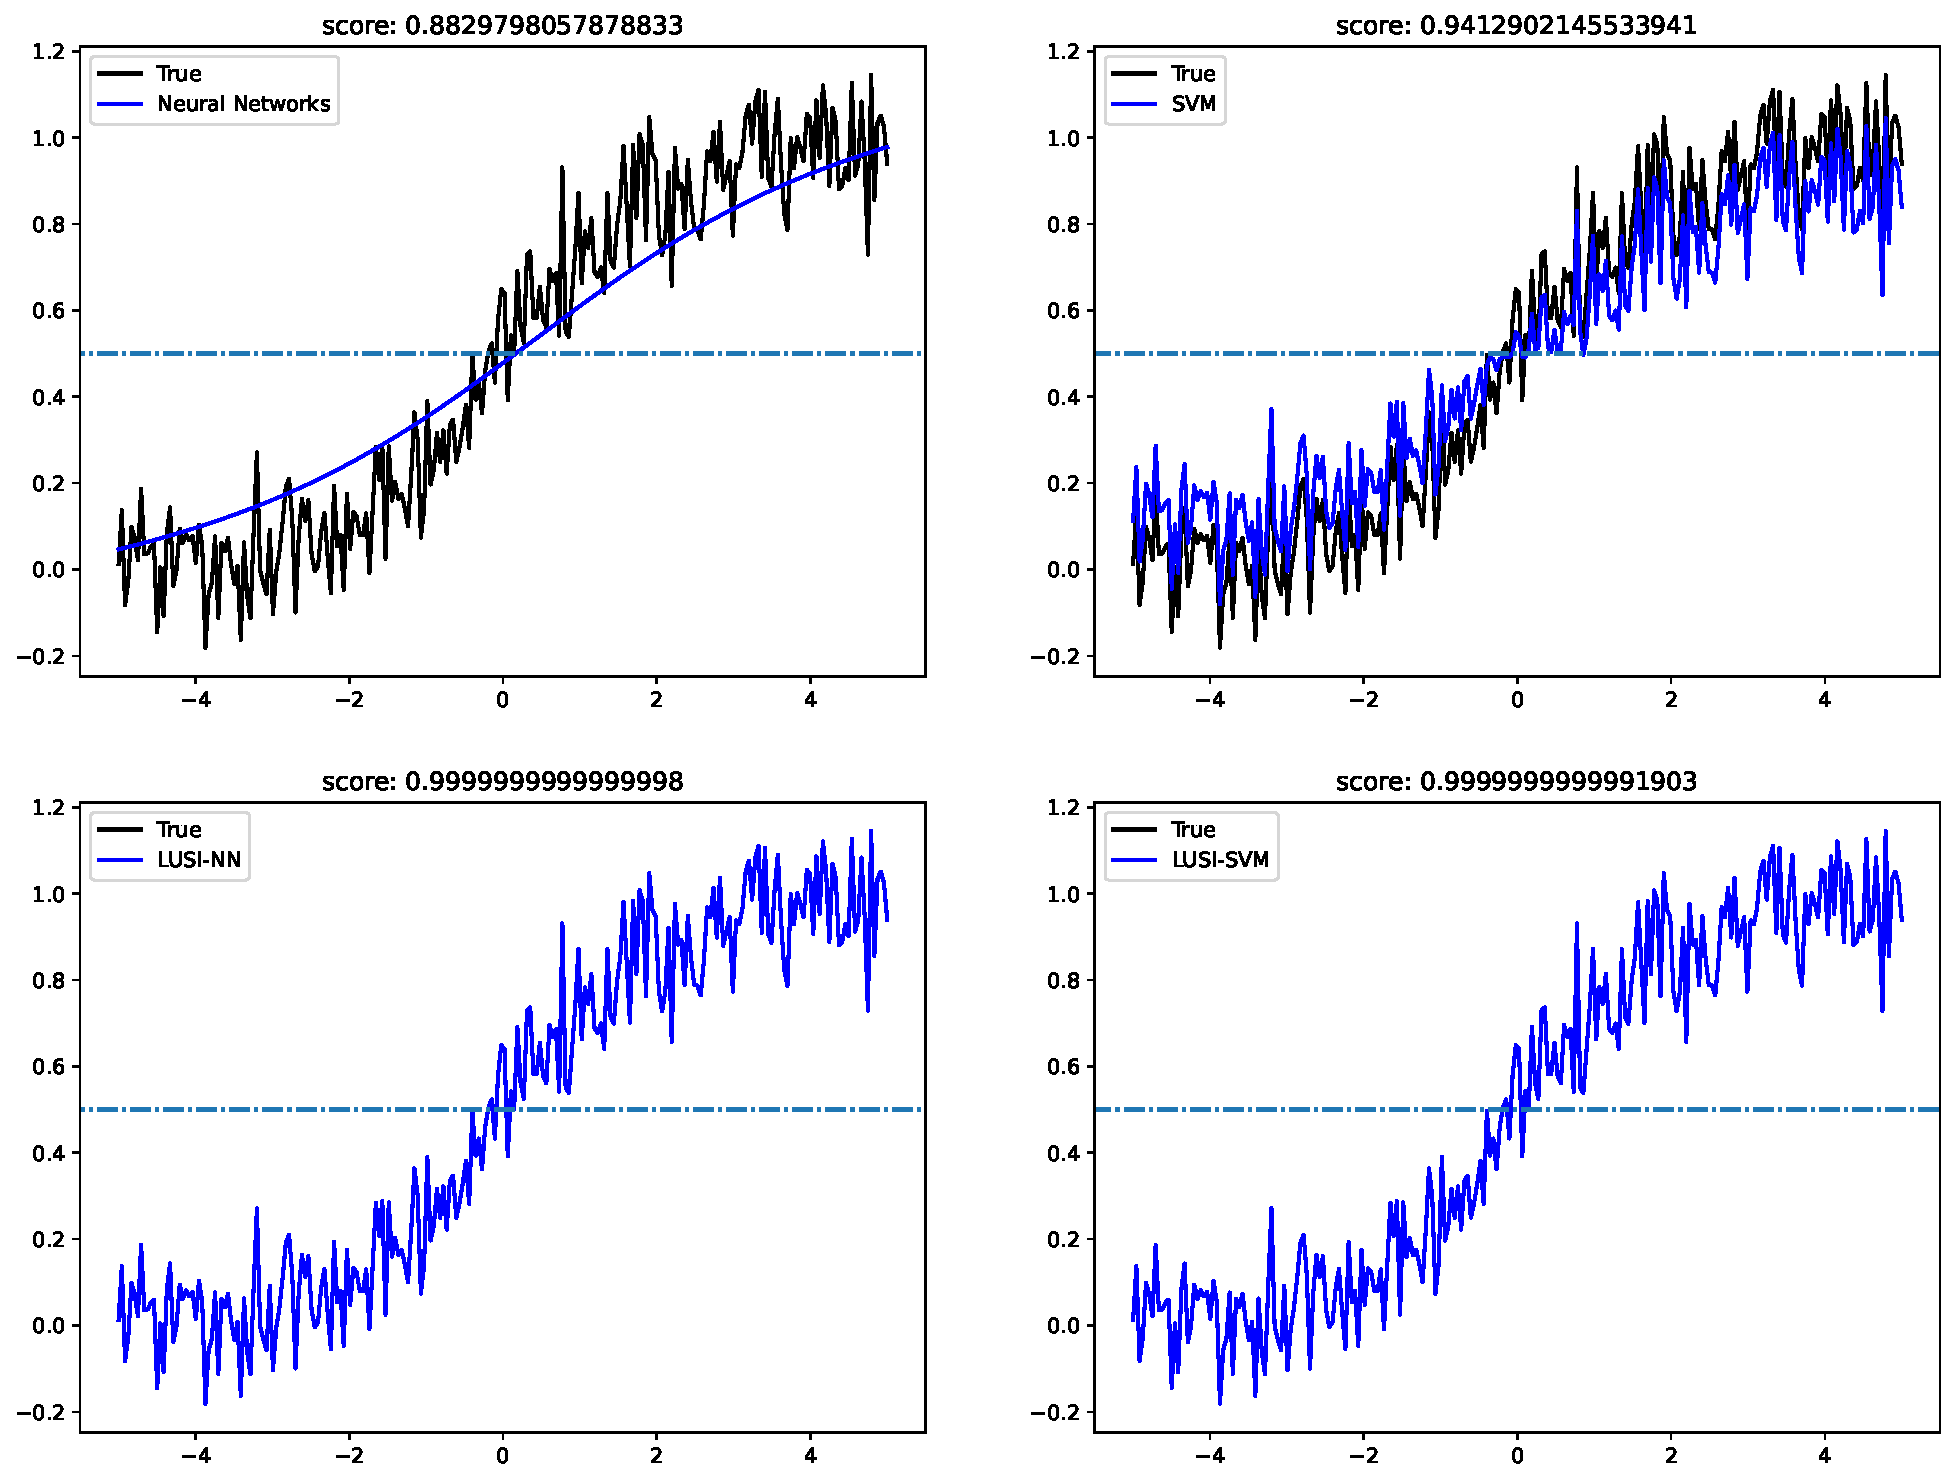
\includegraphics[width=1\linewidth]{Imgs/LUSI_regression_NN_SVM.pdf}
\end{figure}
\end{frame}

\begin{frame}
\begin{figure}[htbp]
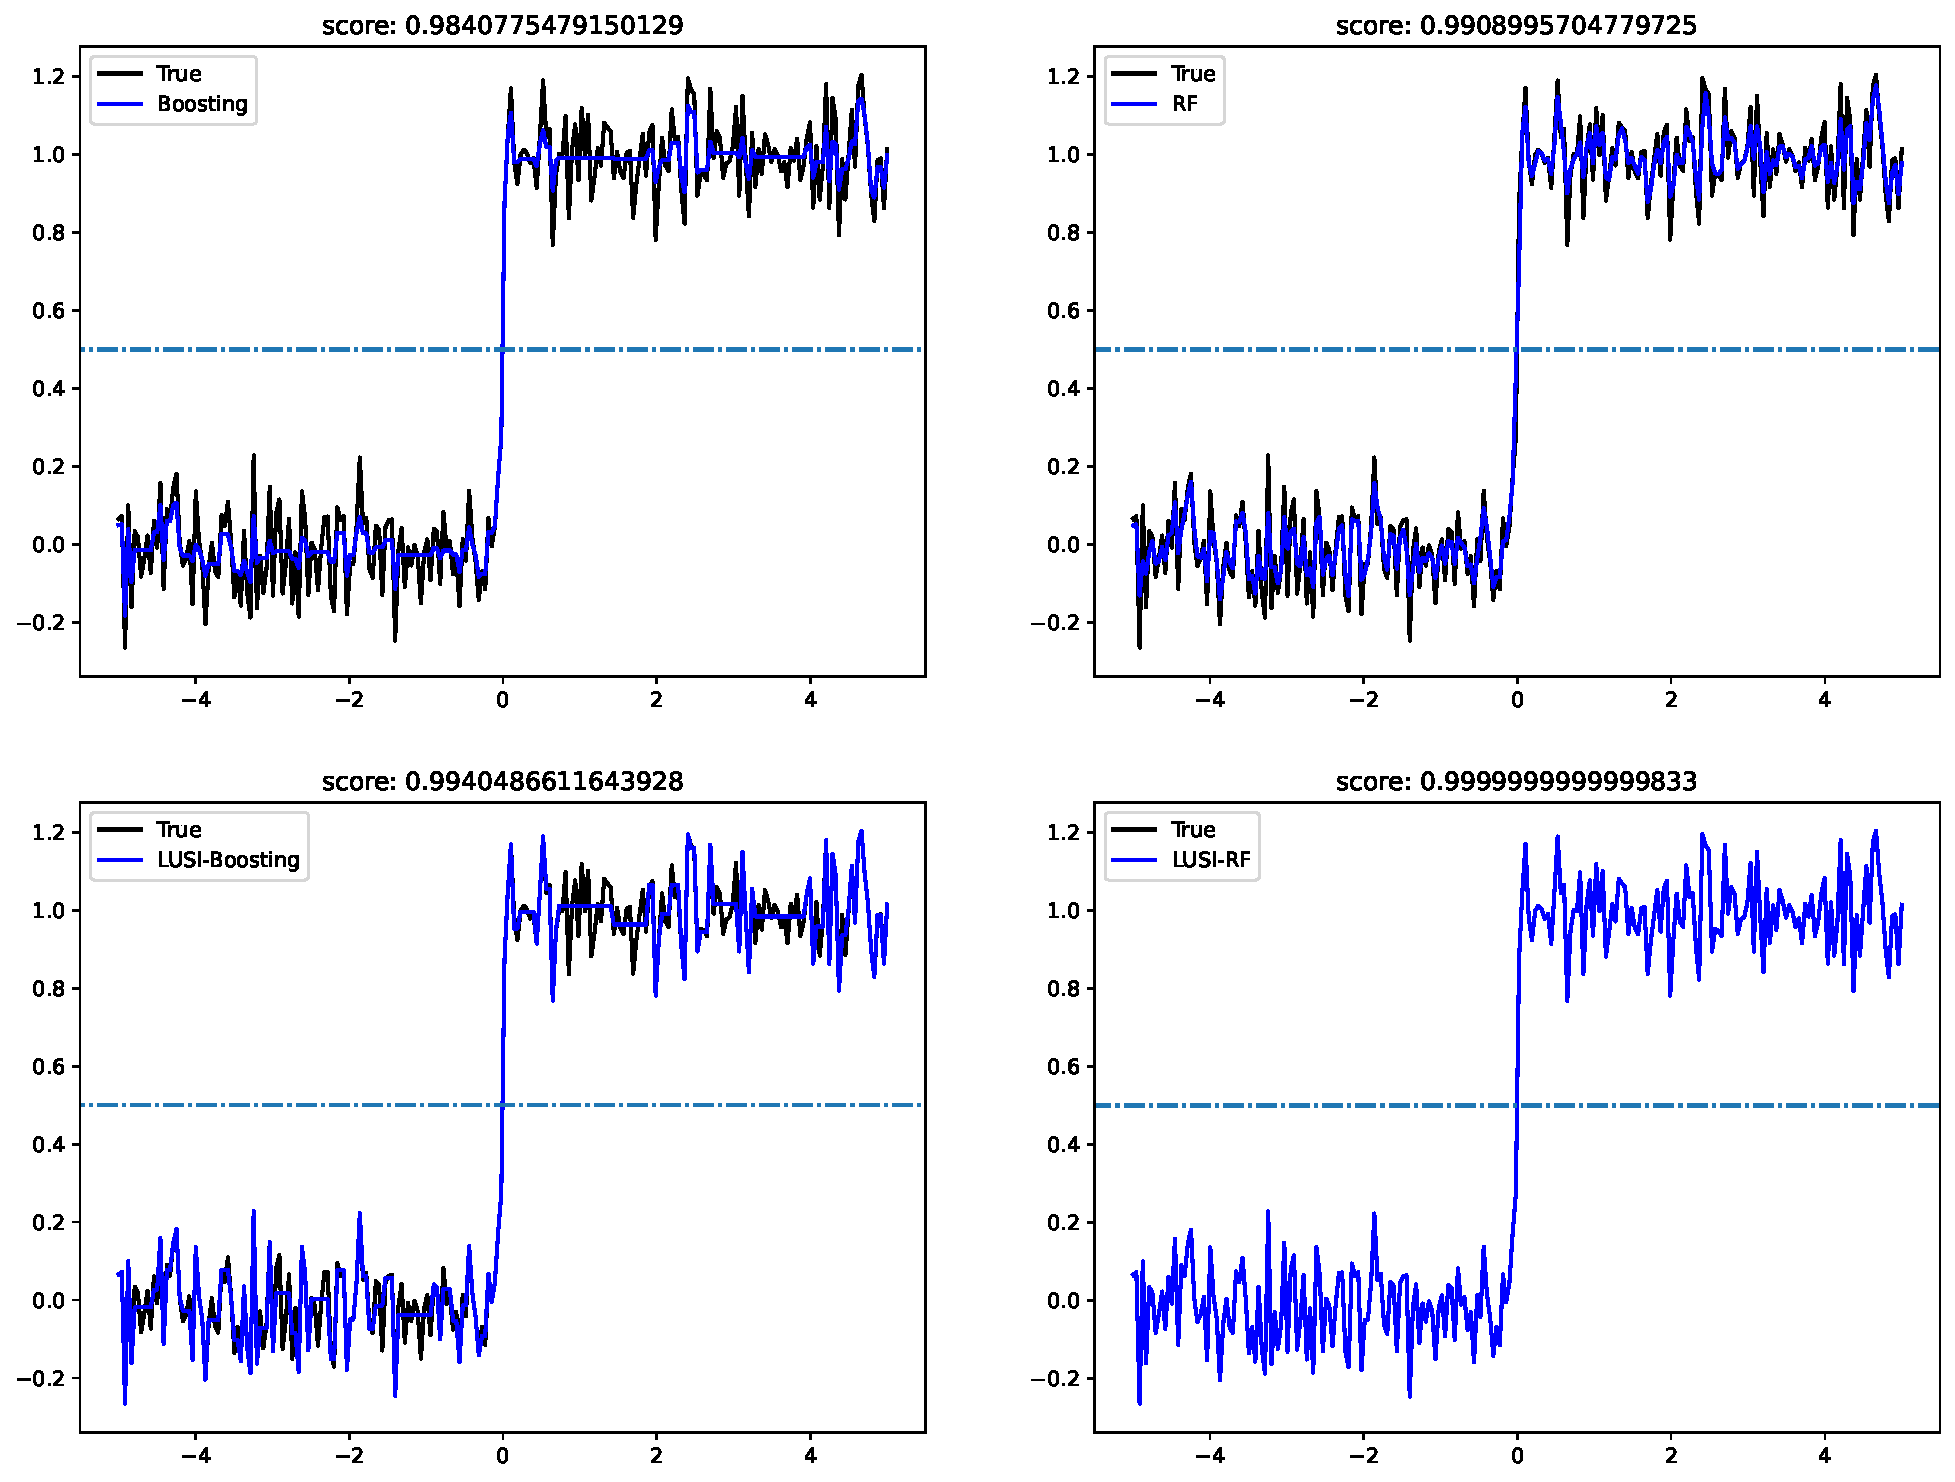
\includegraphics[width=1\linewidth]{Imgs/LUSI_regression_Boosting_RF.pdf}
\end{figure}
\end{frame}

\begin{frame}{成果}
\begin{enumerate}
\item \textbf{Zepu Xi}, Hongbo Chen, Xiaoqian Chen, Wen Yao. Mondrian Conformal Prediction of Boosting for Swarm Behavior Recognition. 2022 IEEE International Conference on Unmanned Systems ({IEEE ICUS}). 2022. (EI会议)
\item \textbf{Zepu Xi}. Distributions-free Martingale Test Distributions-shift for Swarm Behavior Prediction. 2022 International Joint Conference on Neural Networks (IJCNN). 2022. (CCF-C, 人工智能学术A类会议)
\item \textbf{Zepu Xi}, Xuebin Zhuang, Hongbo Chen. Conformal Prediction for Hypersonic Flight Vehicle Classification. Proceedings of the 12th Symposium on Conformal and Probabilistic Prediction with Applications (COPA). PMLR. 2022. (Conformal Prediction 指定会议)
\item \textbf{Zepu Xi}, Xuebin Zhuang, Hongbo Chen. Post-selection Inference, with Application to Autoregressive Processes. 2021 International Conference on Mechanical, Aerospace and Automotive Engineering (CMAAE), 2021. (EI会议)
\end{enumerate}
\end{frame}

\begin{frame}[plain,noframenumbering]
\vspace{0.12\textheight}\centering\Huge{谢谢各位老师!}\hspace{0em}
\end{frame}

\end{document} 